The focus of the analysis is the processing of the reports submitted. A diagram of this can be found in [Figure 3 - State Diagram]. By modeling it using Alloy, we can verify the following points:

\begin{itemize}
    \item All possible scenarios of a report analysis are covered by our established definitions.
    \item There is no overlap of report definitions. An overlap would make the definitions ambiguous and the final result would ultimately depend on the implementation.
    \item All definitions of the result of a report analysis are possible with the given assumptions and constraints.
\end{itemize}

\noindent\fbox{%
    \parbox{\dimexpr\textwidth-10pt}{%
    \textbf{Clarifications} \\
    Some aspects of the report are ignored (such as time, location and the user that submitted it) as they are not constrained in any way and do not affect the analysis of the report. \\
The rest of the system is not contemplated as it is fairly straightforward and its properties can be trivially checked (for example, no two users share the same username/email).
    }%
}


\subsection{The model}

\lstinputlisting[language=alloy]{../alloy/model.als}
\lstinputlisting[language=alloy]{../alloy/reportDefinitions.als}

\subsection{Assertions and checks}

\lstinputlisting[language=alloy]{../alloy/assertions.als}
\begin{figure}[H]
    \centering
    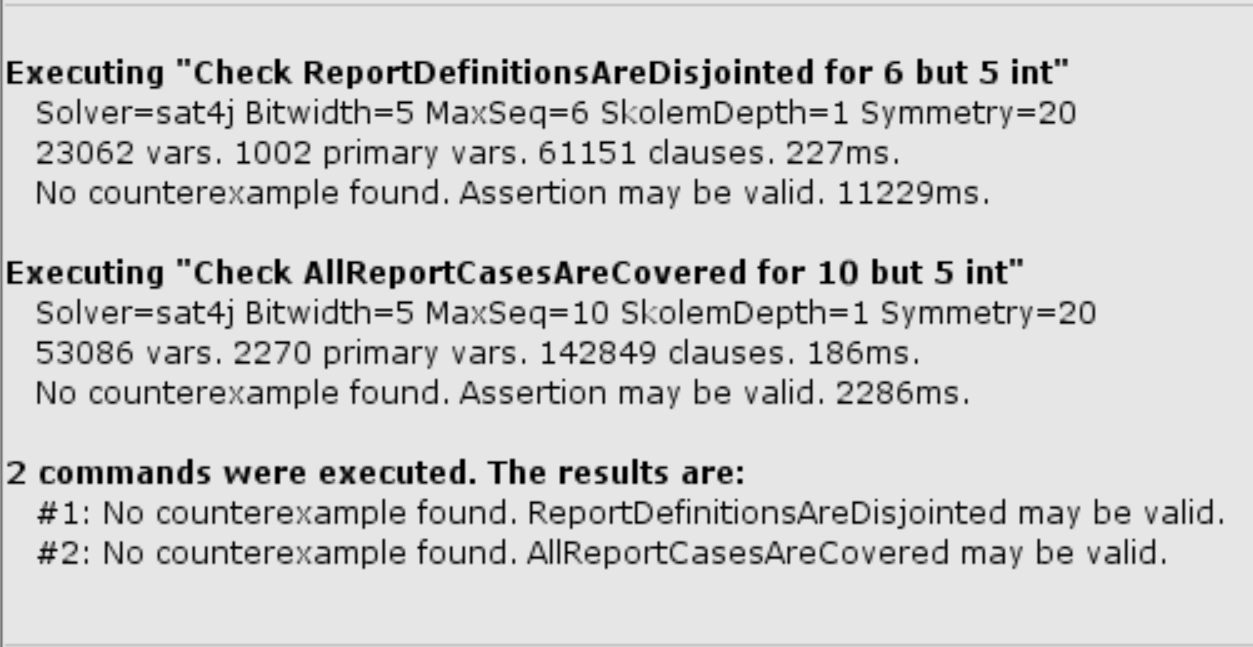
\includegraphics[width=\textwidth]{Images/alloy/assertion-results.png}
    \caption{\label{fig:alloy}Alloy - Assertion results.}
\end{figure}

\subsection{World generation}

\lstinputlisting[language=alloy]{../alloy/worldgen.als}

\begin{figure}[H]
    \centering
    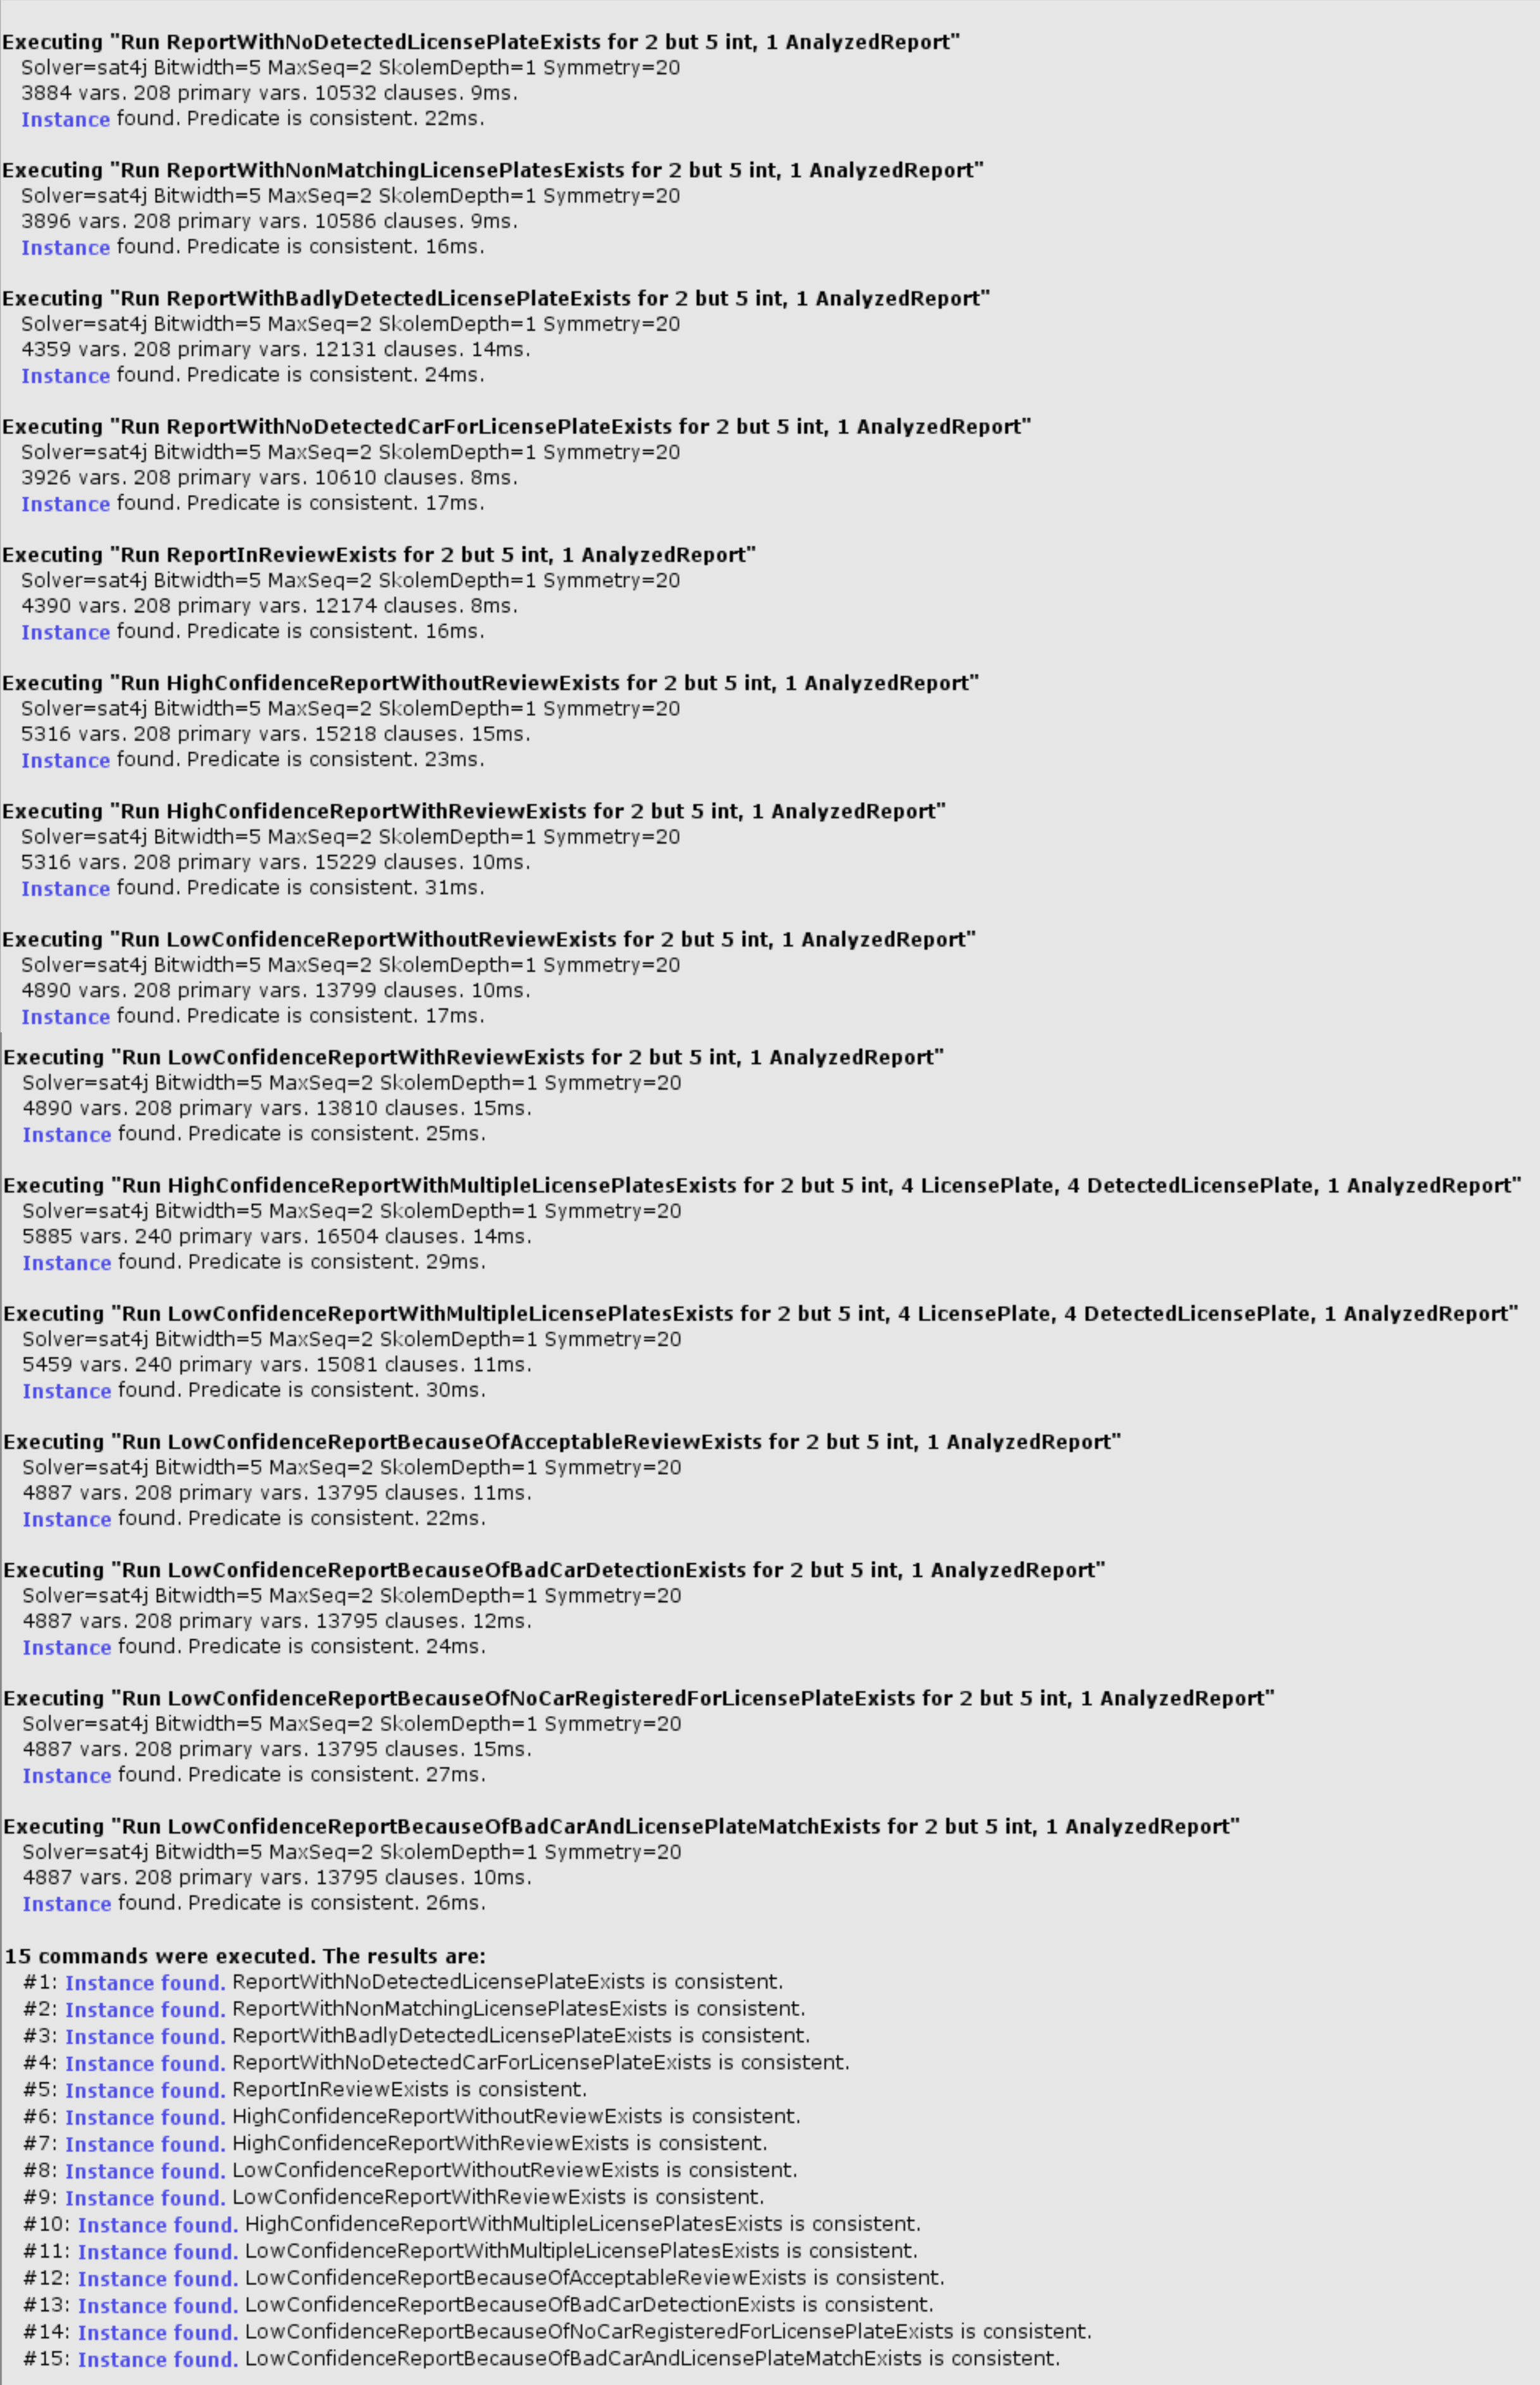
\includegraphics[width=0.97\textwidth]{Images/alloy/worldgen.png}
    \caption{\label{fig:alloy}Alloy - World generation results.}
\end{figure}

\begin{figure}[H]
    \centering
    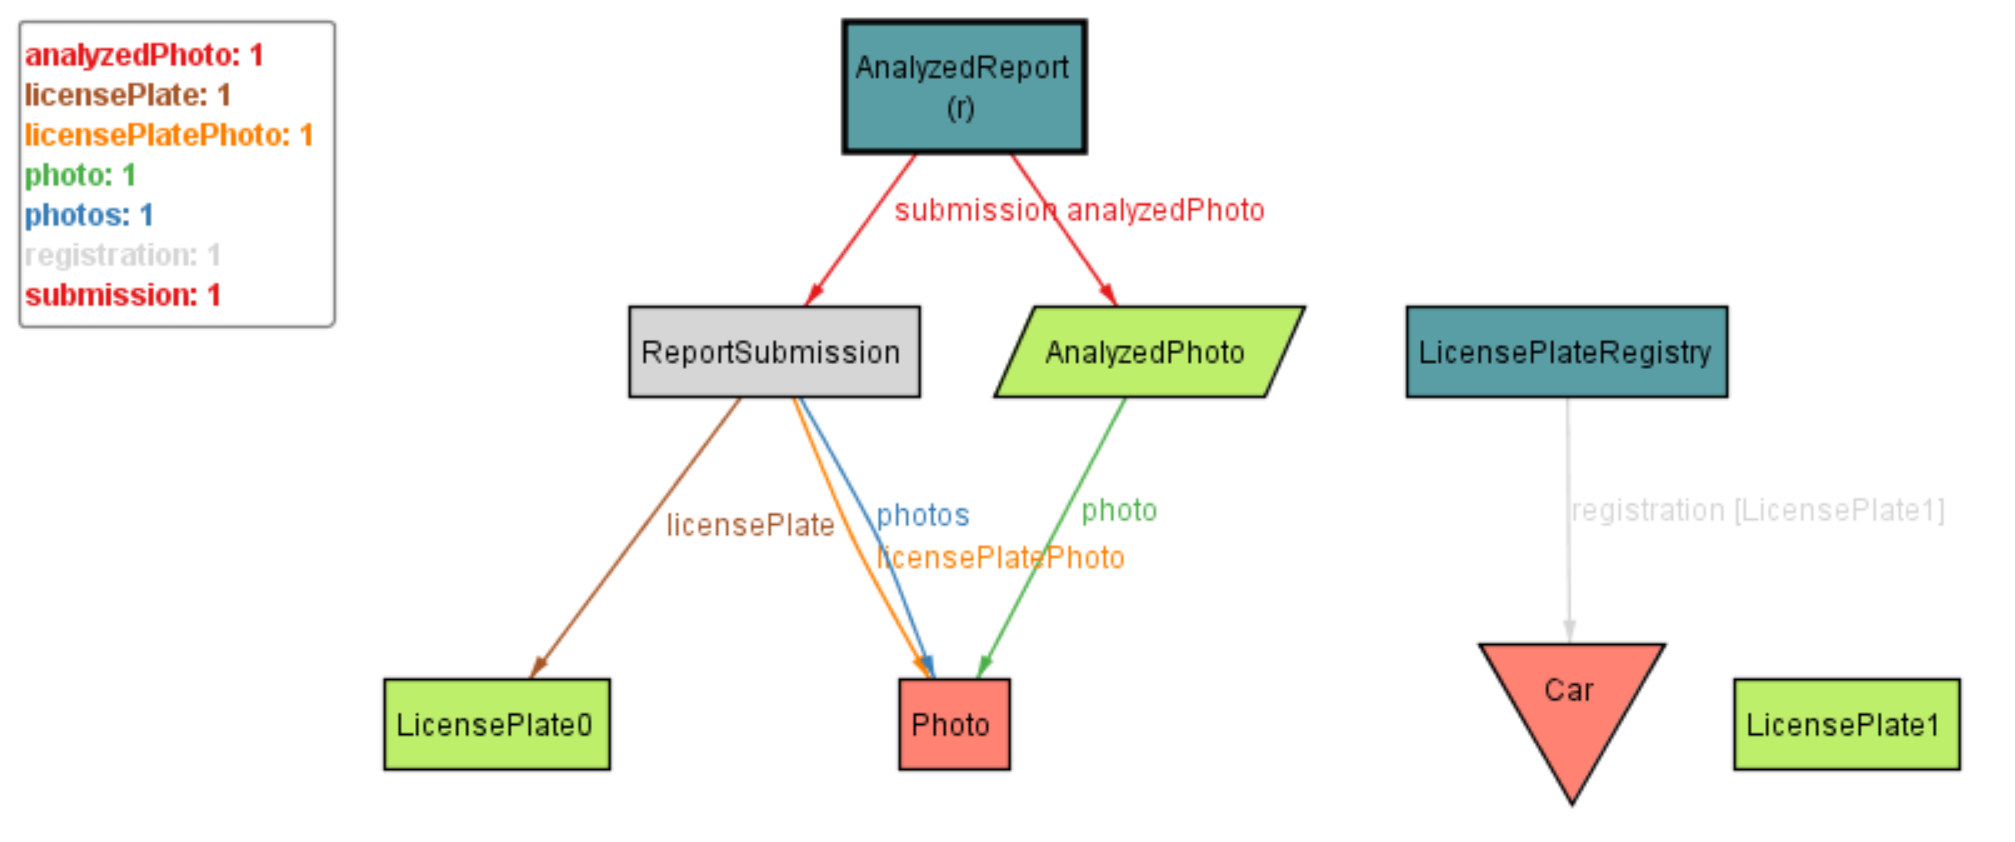
\includegraphics[width=\textwidth]{Images/alloy/1.png}
    \caption{\label{fig:alloy}Alloy - World: Report with no detected license plate.}
\end{figure}

\begin{figure}[H]
    \centering
    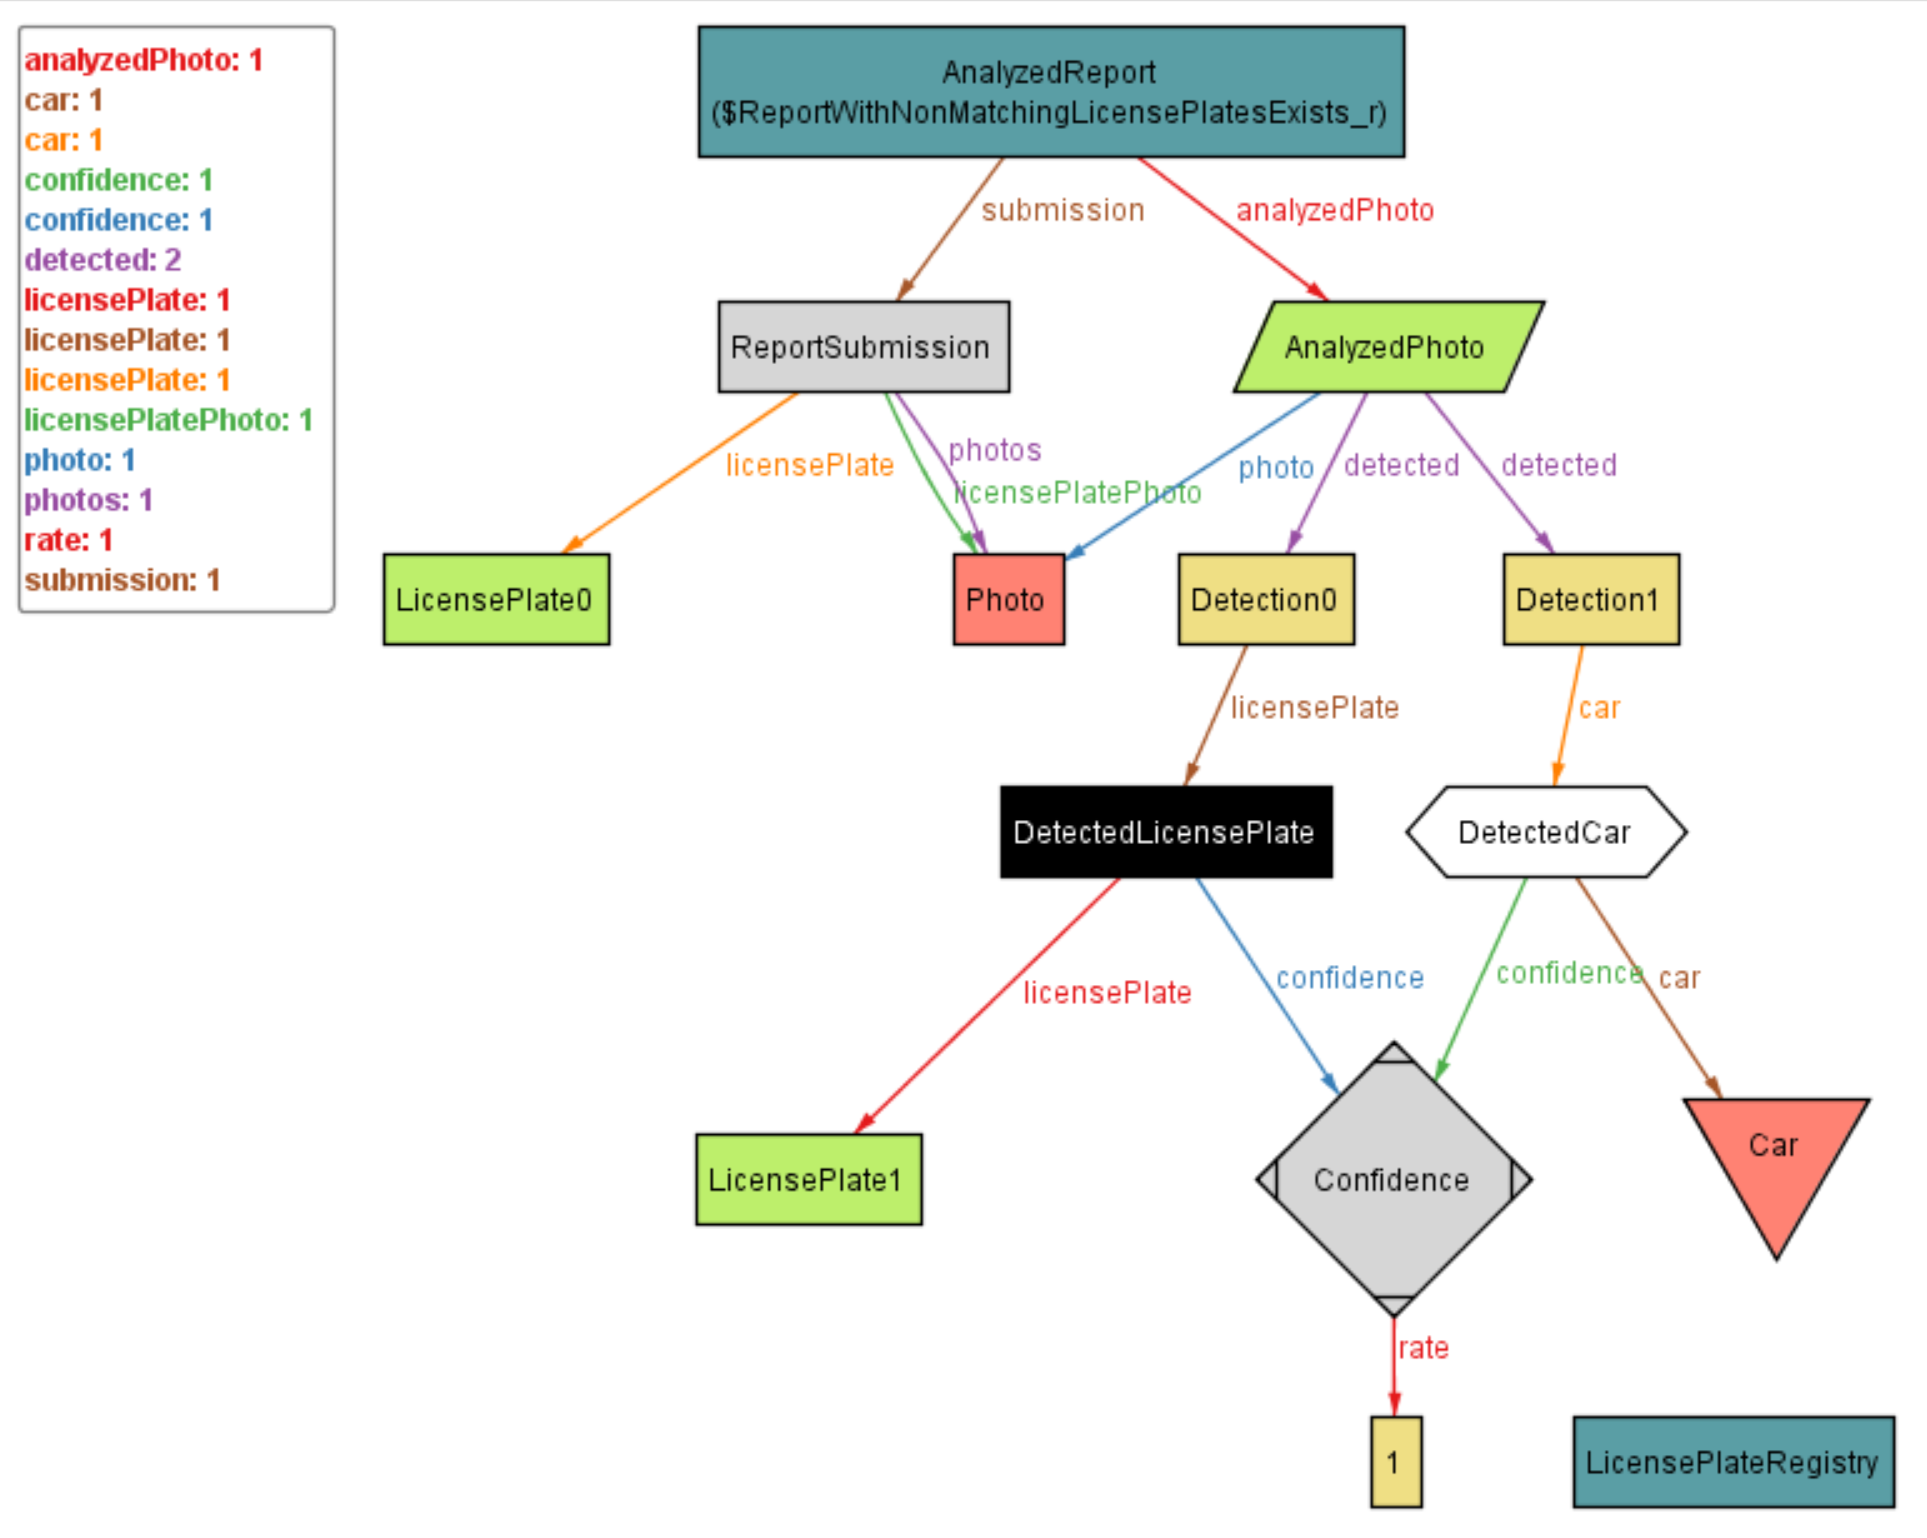
\includegraphics[width=\textwidth]{Images/alloy/2.png}
    \caption{\label{fig:alloy}Alloy - World: Report with non matching detected and submitted license plates.}
\end{figure}

\begin{figure}[H]
    \centering
    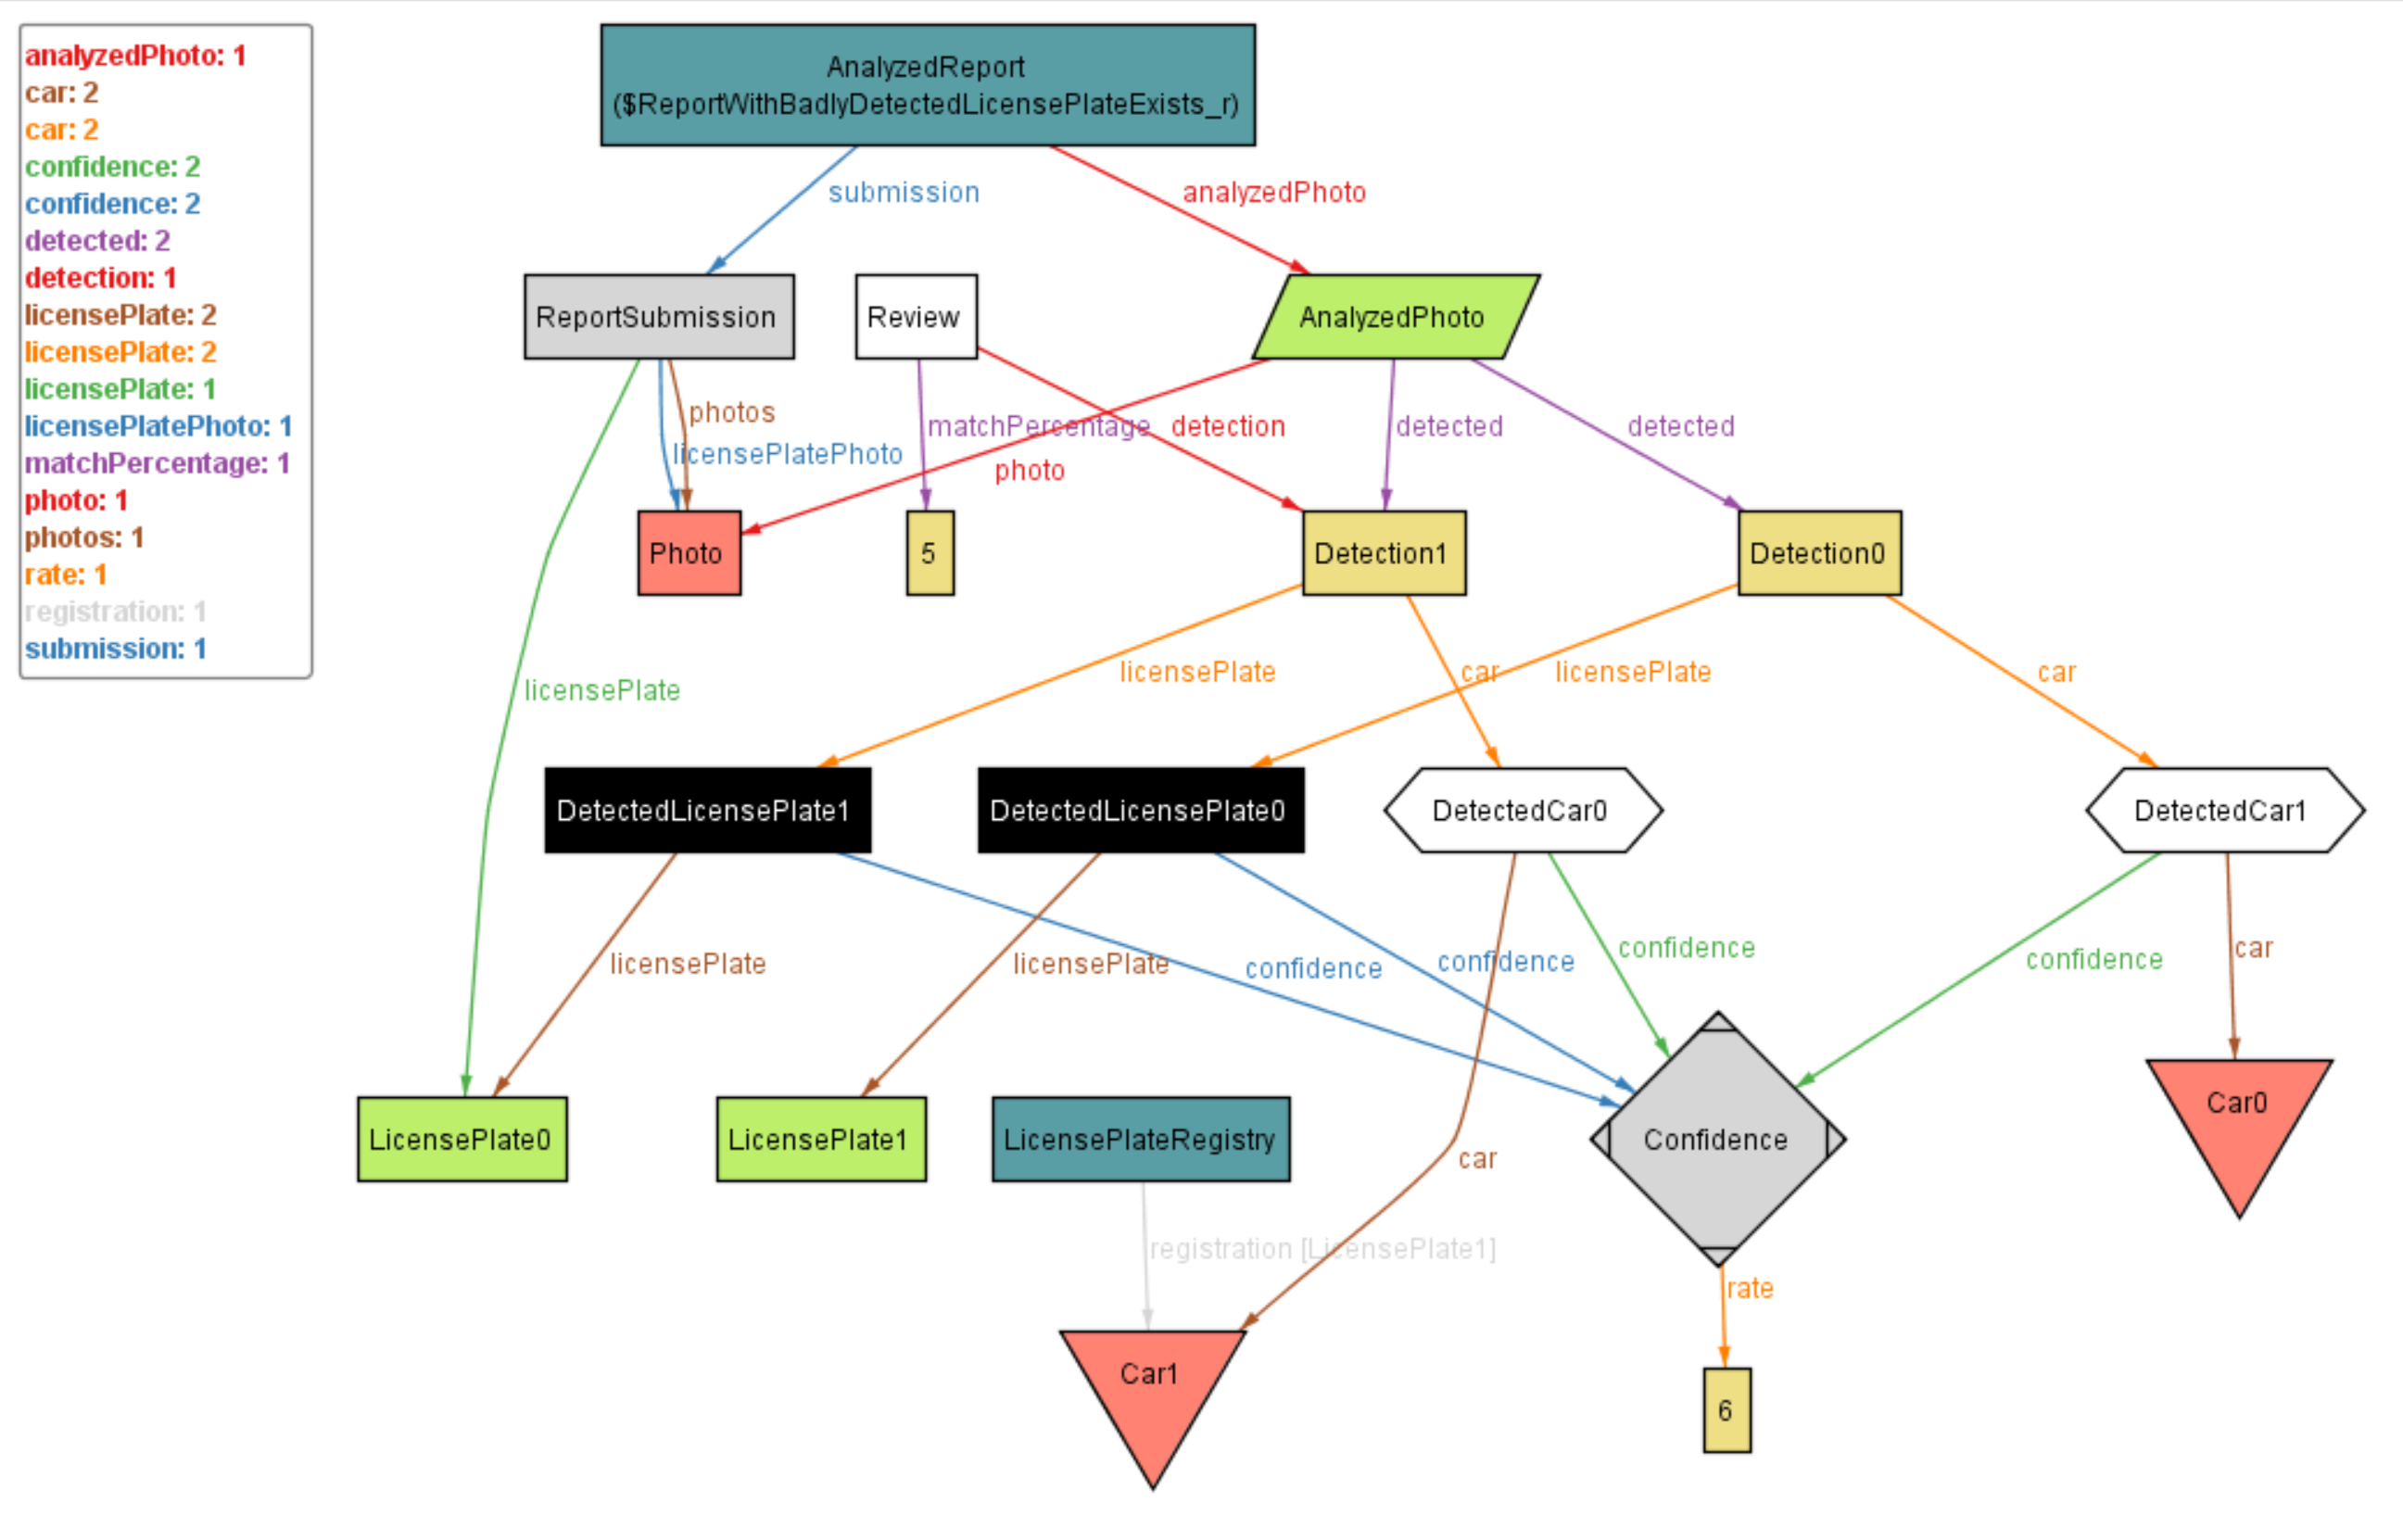
\includegraphics[width=\textwidth]{Images/alloy/3.png}
    \caption{\label{fig:alloy}Alloy - World: Report with badly detected license plate.}
\end{figure}

\begin{figure}[H]
    \centering
    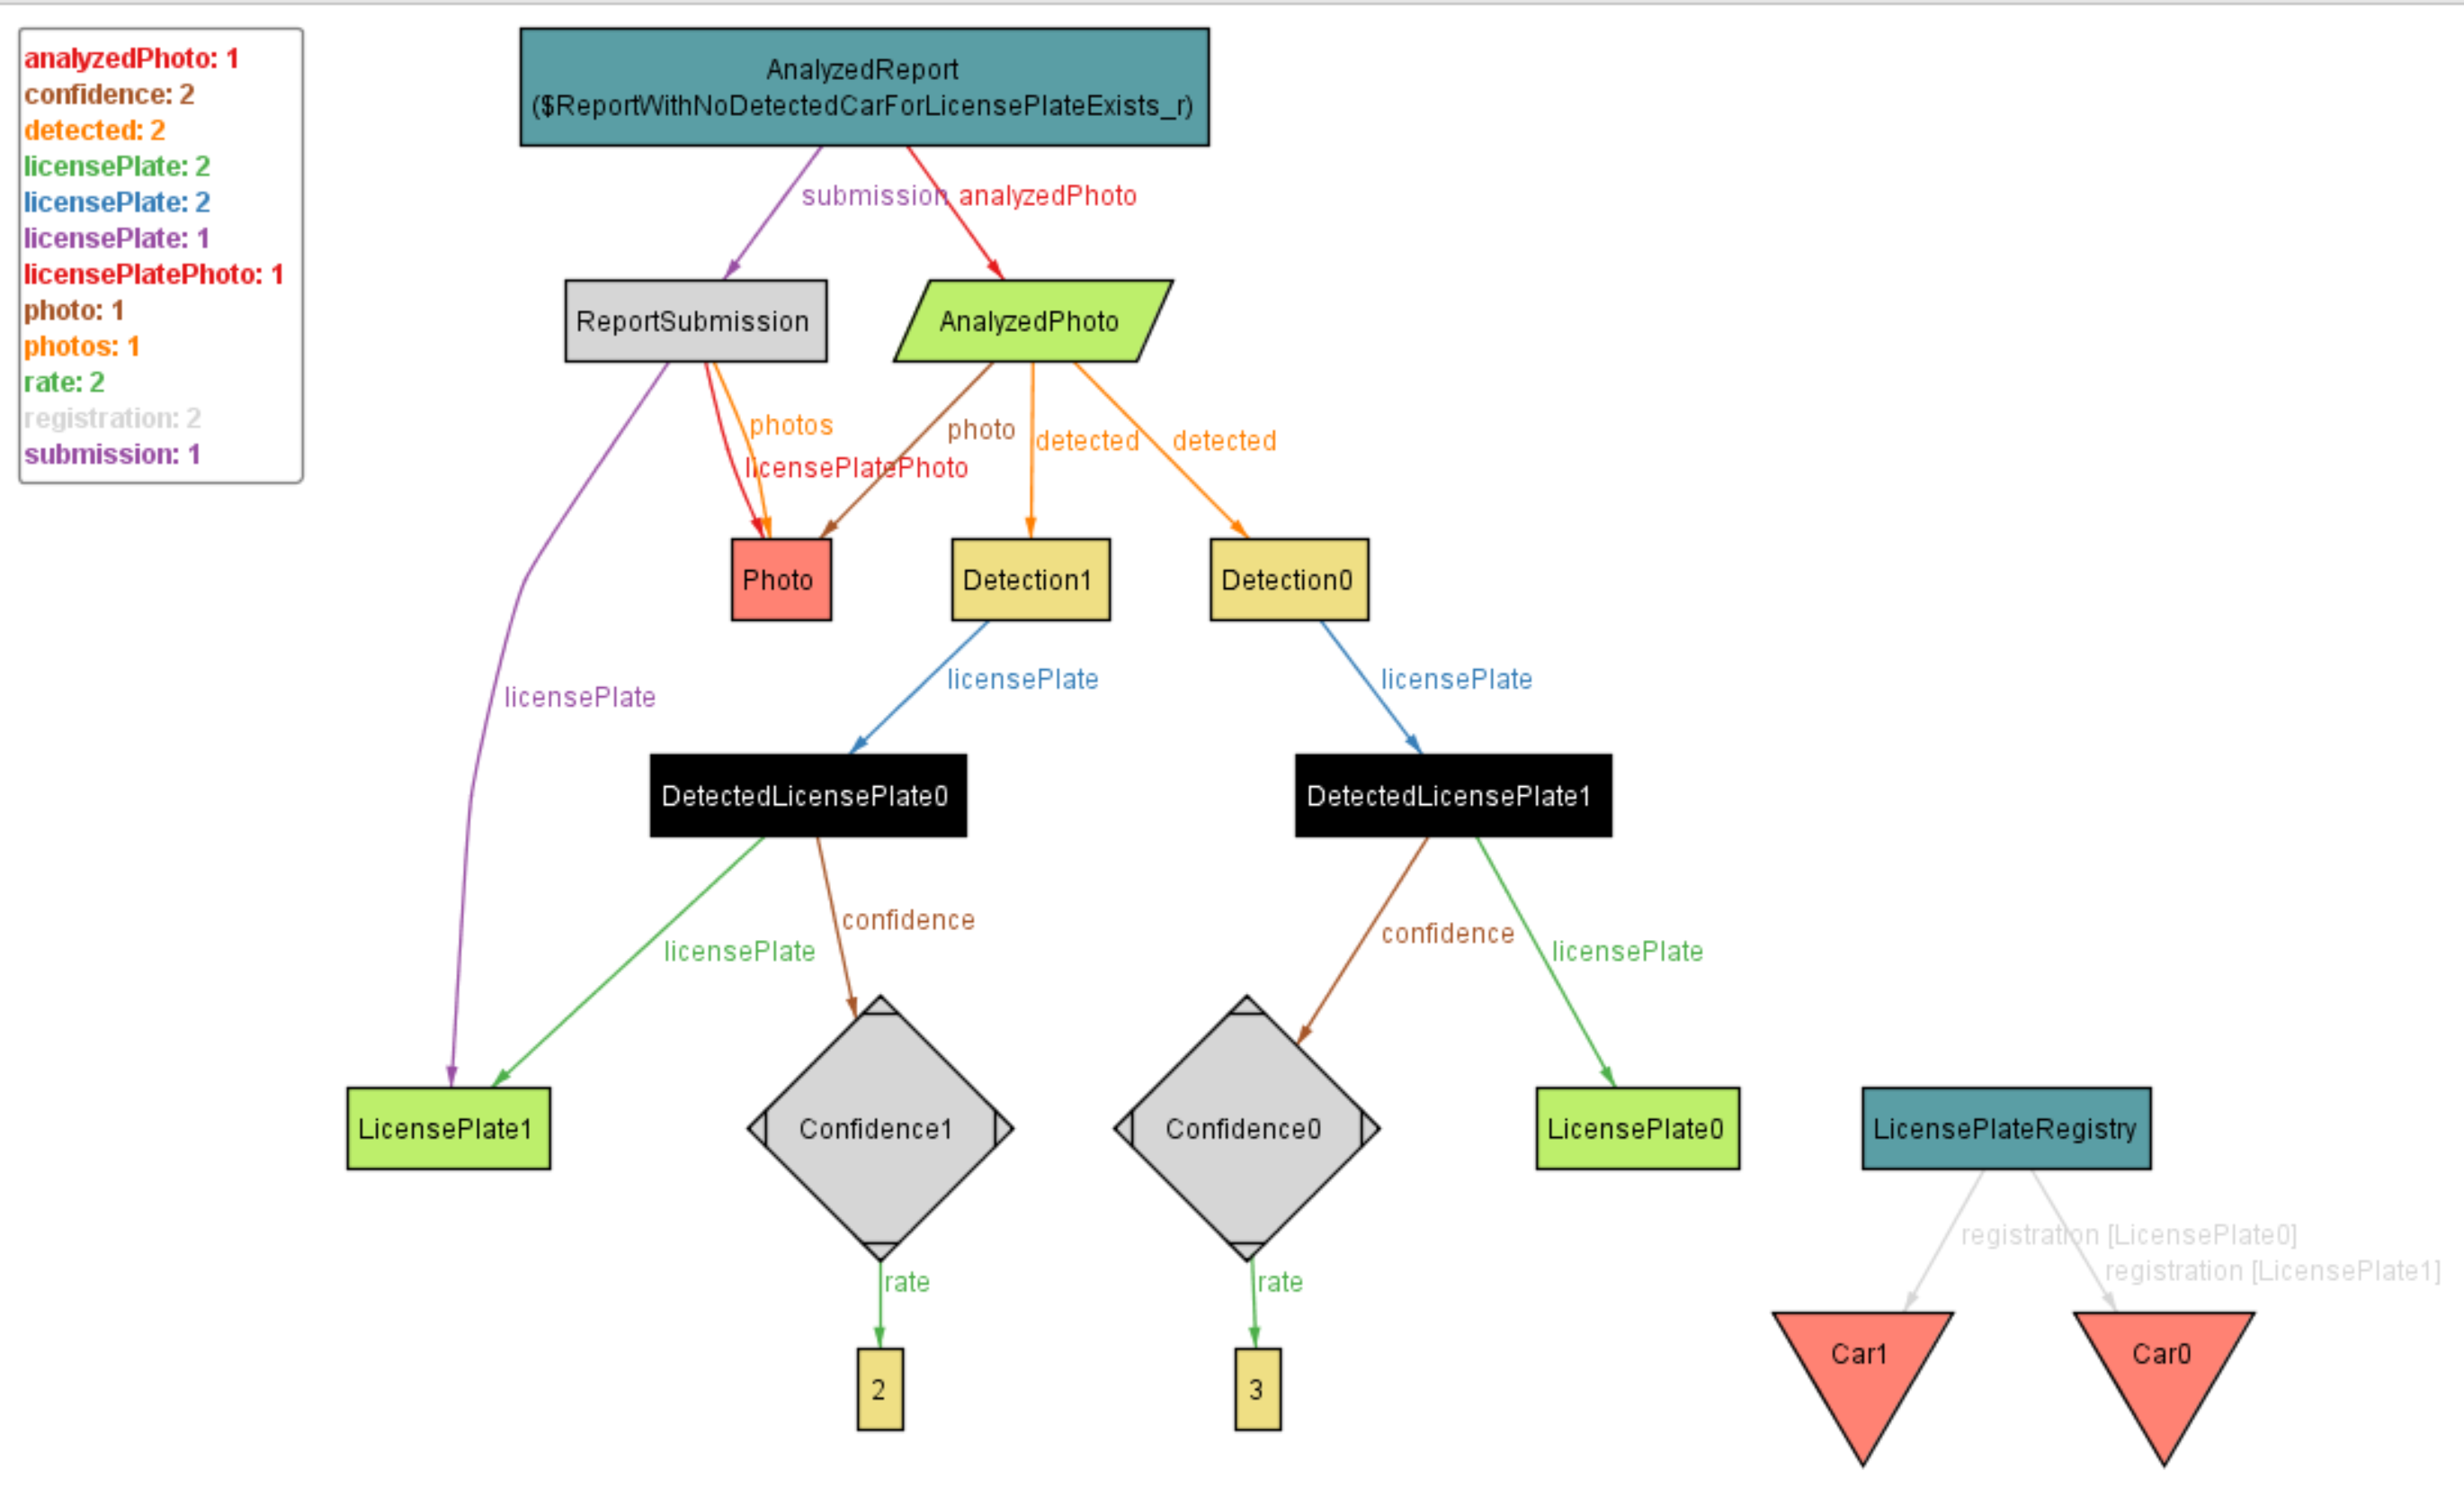
\includegraphics[width=\textwidth]{Images/alloy/4.png}
    \caption{\label{fig:alloy}Alloy - World: Report with no detected car for license plate.}
\end{figure}

\begin{figure}[H]
    \centering
    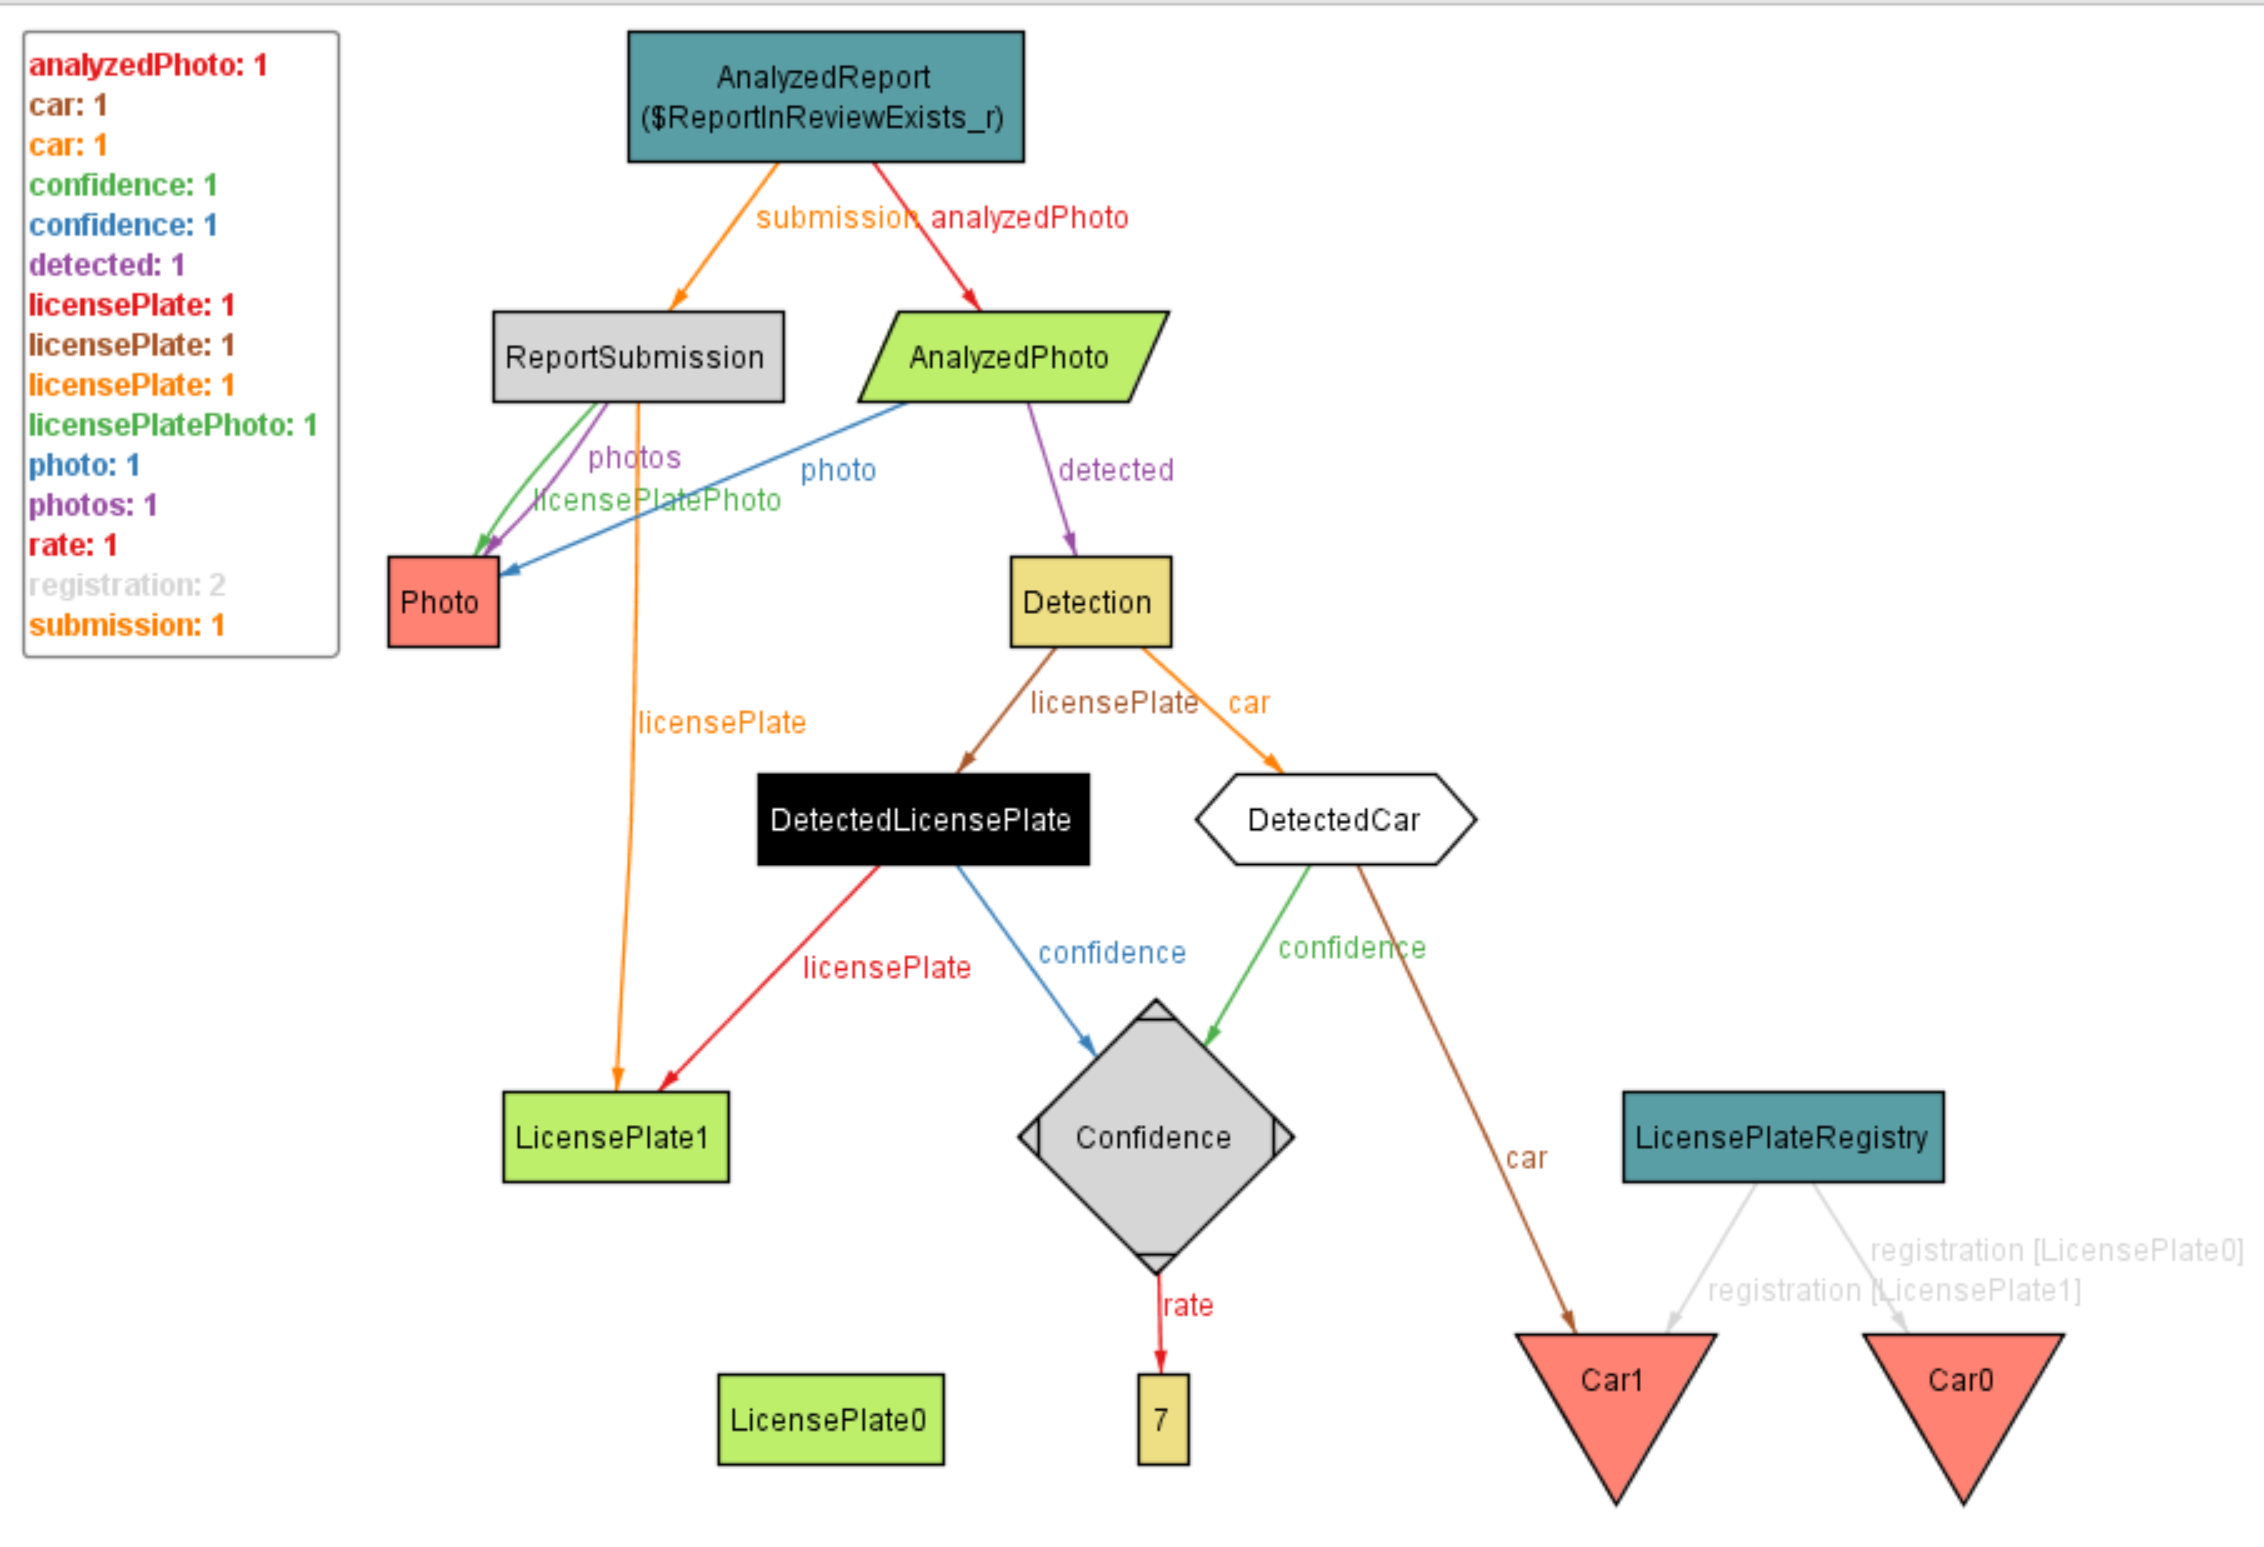
\includegraphics[width=\textwidth]{Images/alloy/5.png}
    \caption{\label{fig:alloy}Alloy - World: Report in review.}
\end{figure}

\begin{figure}[H]
    \centering
    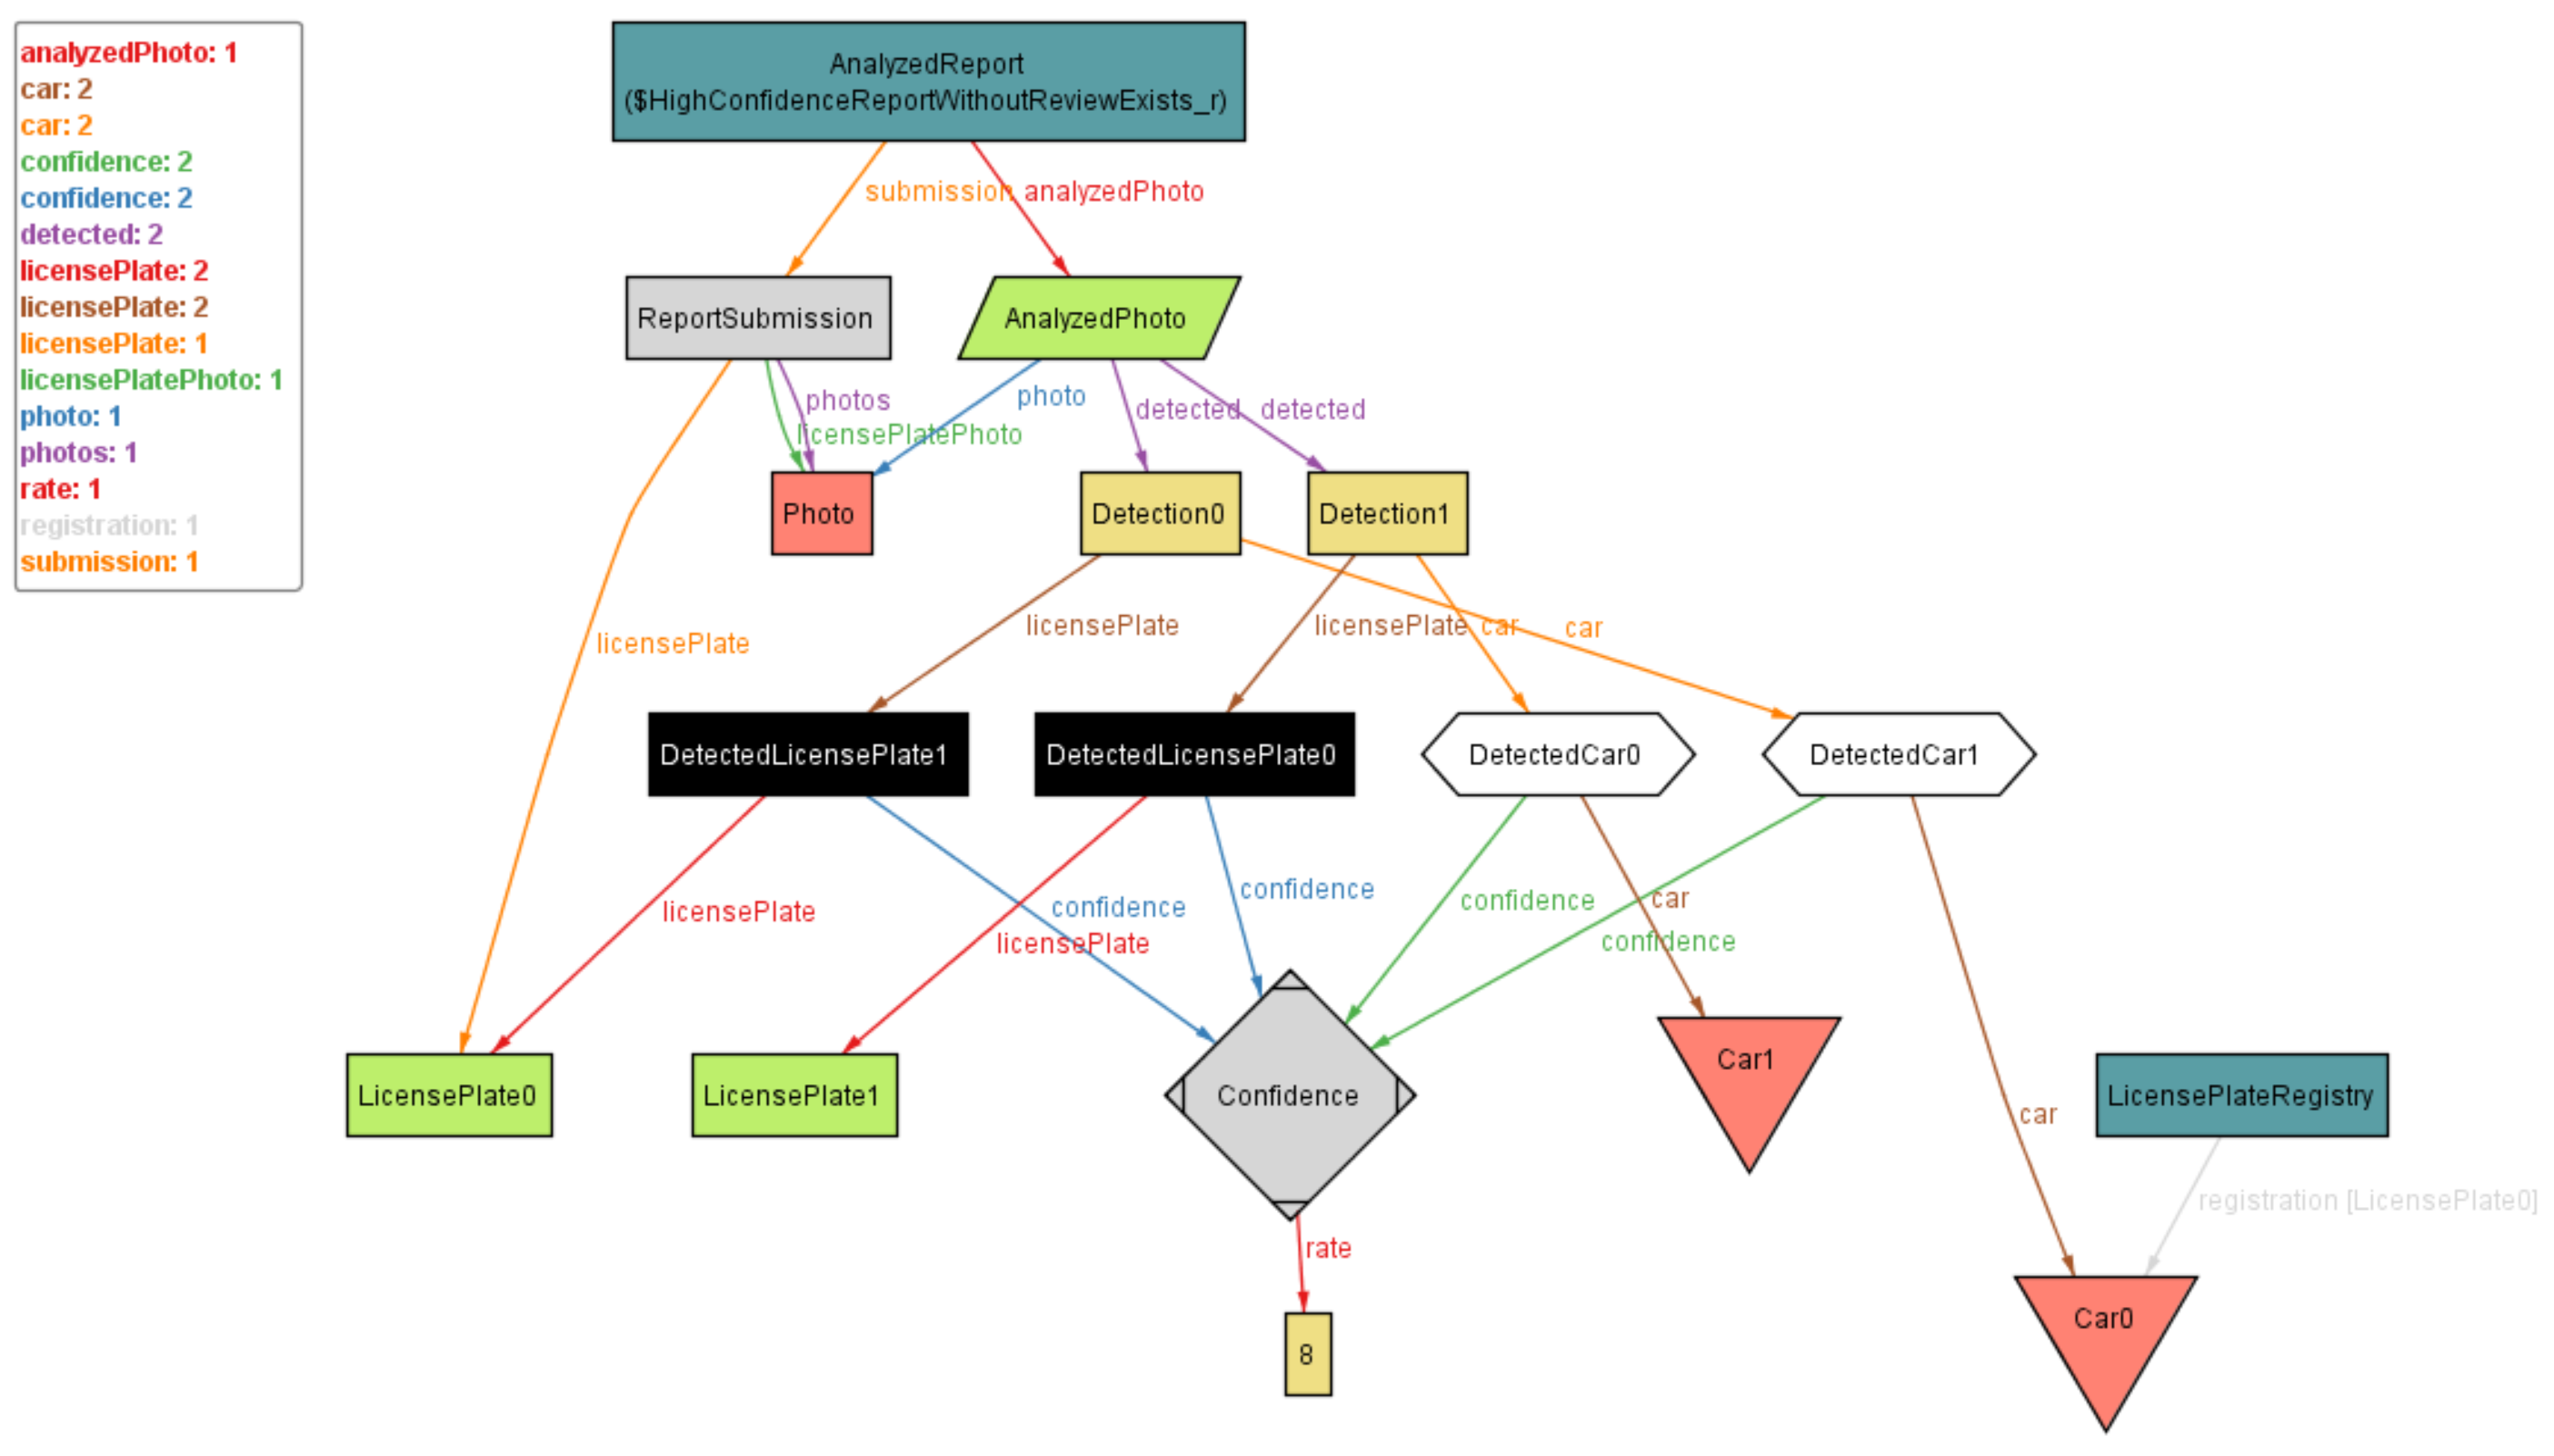
\includegraphics[width=\textwidth]{Images/alloy/6.png}
    \caption{\label{fig:alloy}Alloy - World: High confidence report without a review.}
\end{figure}

\begin{figure}[H]
    \centering
    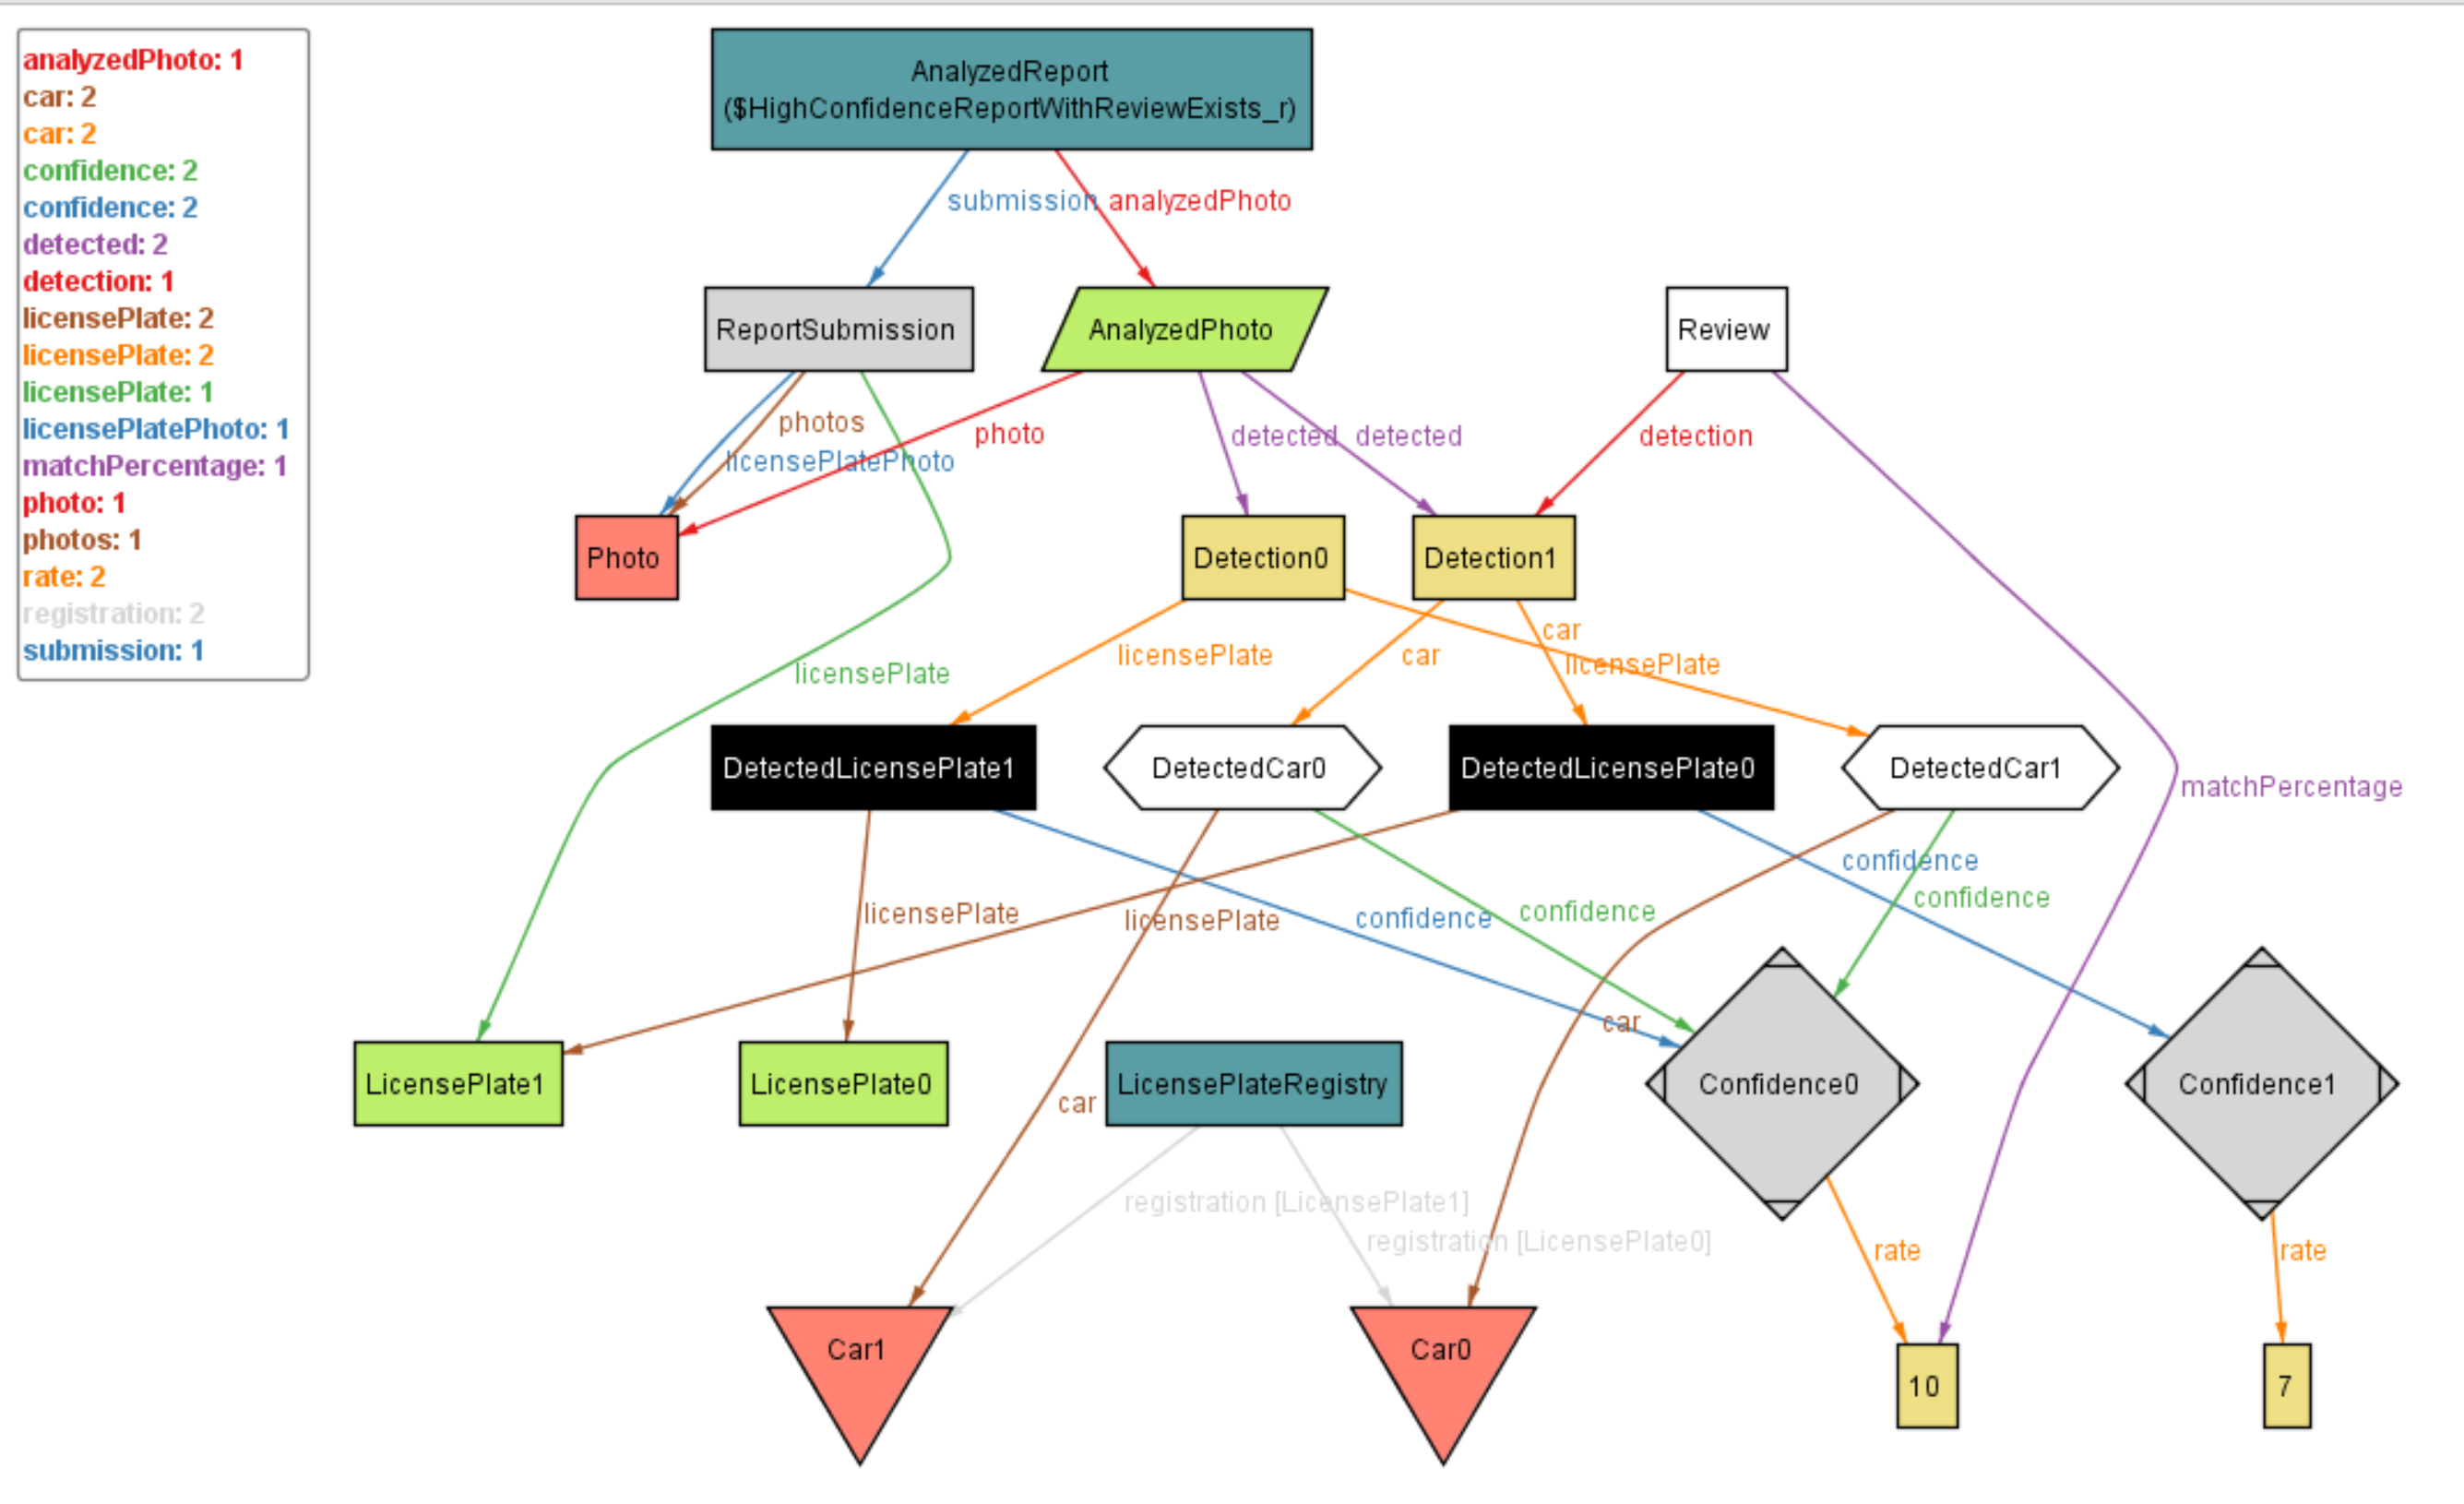
\includegraphics[width=\textwidth]{Images/alloy/7.png}
    \caption{\label{fig:alloy}Alloy - World: High confidence report with a review.}
\end{figure}

\begin{figure}[H]
    \centering
    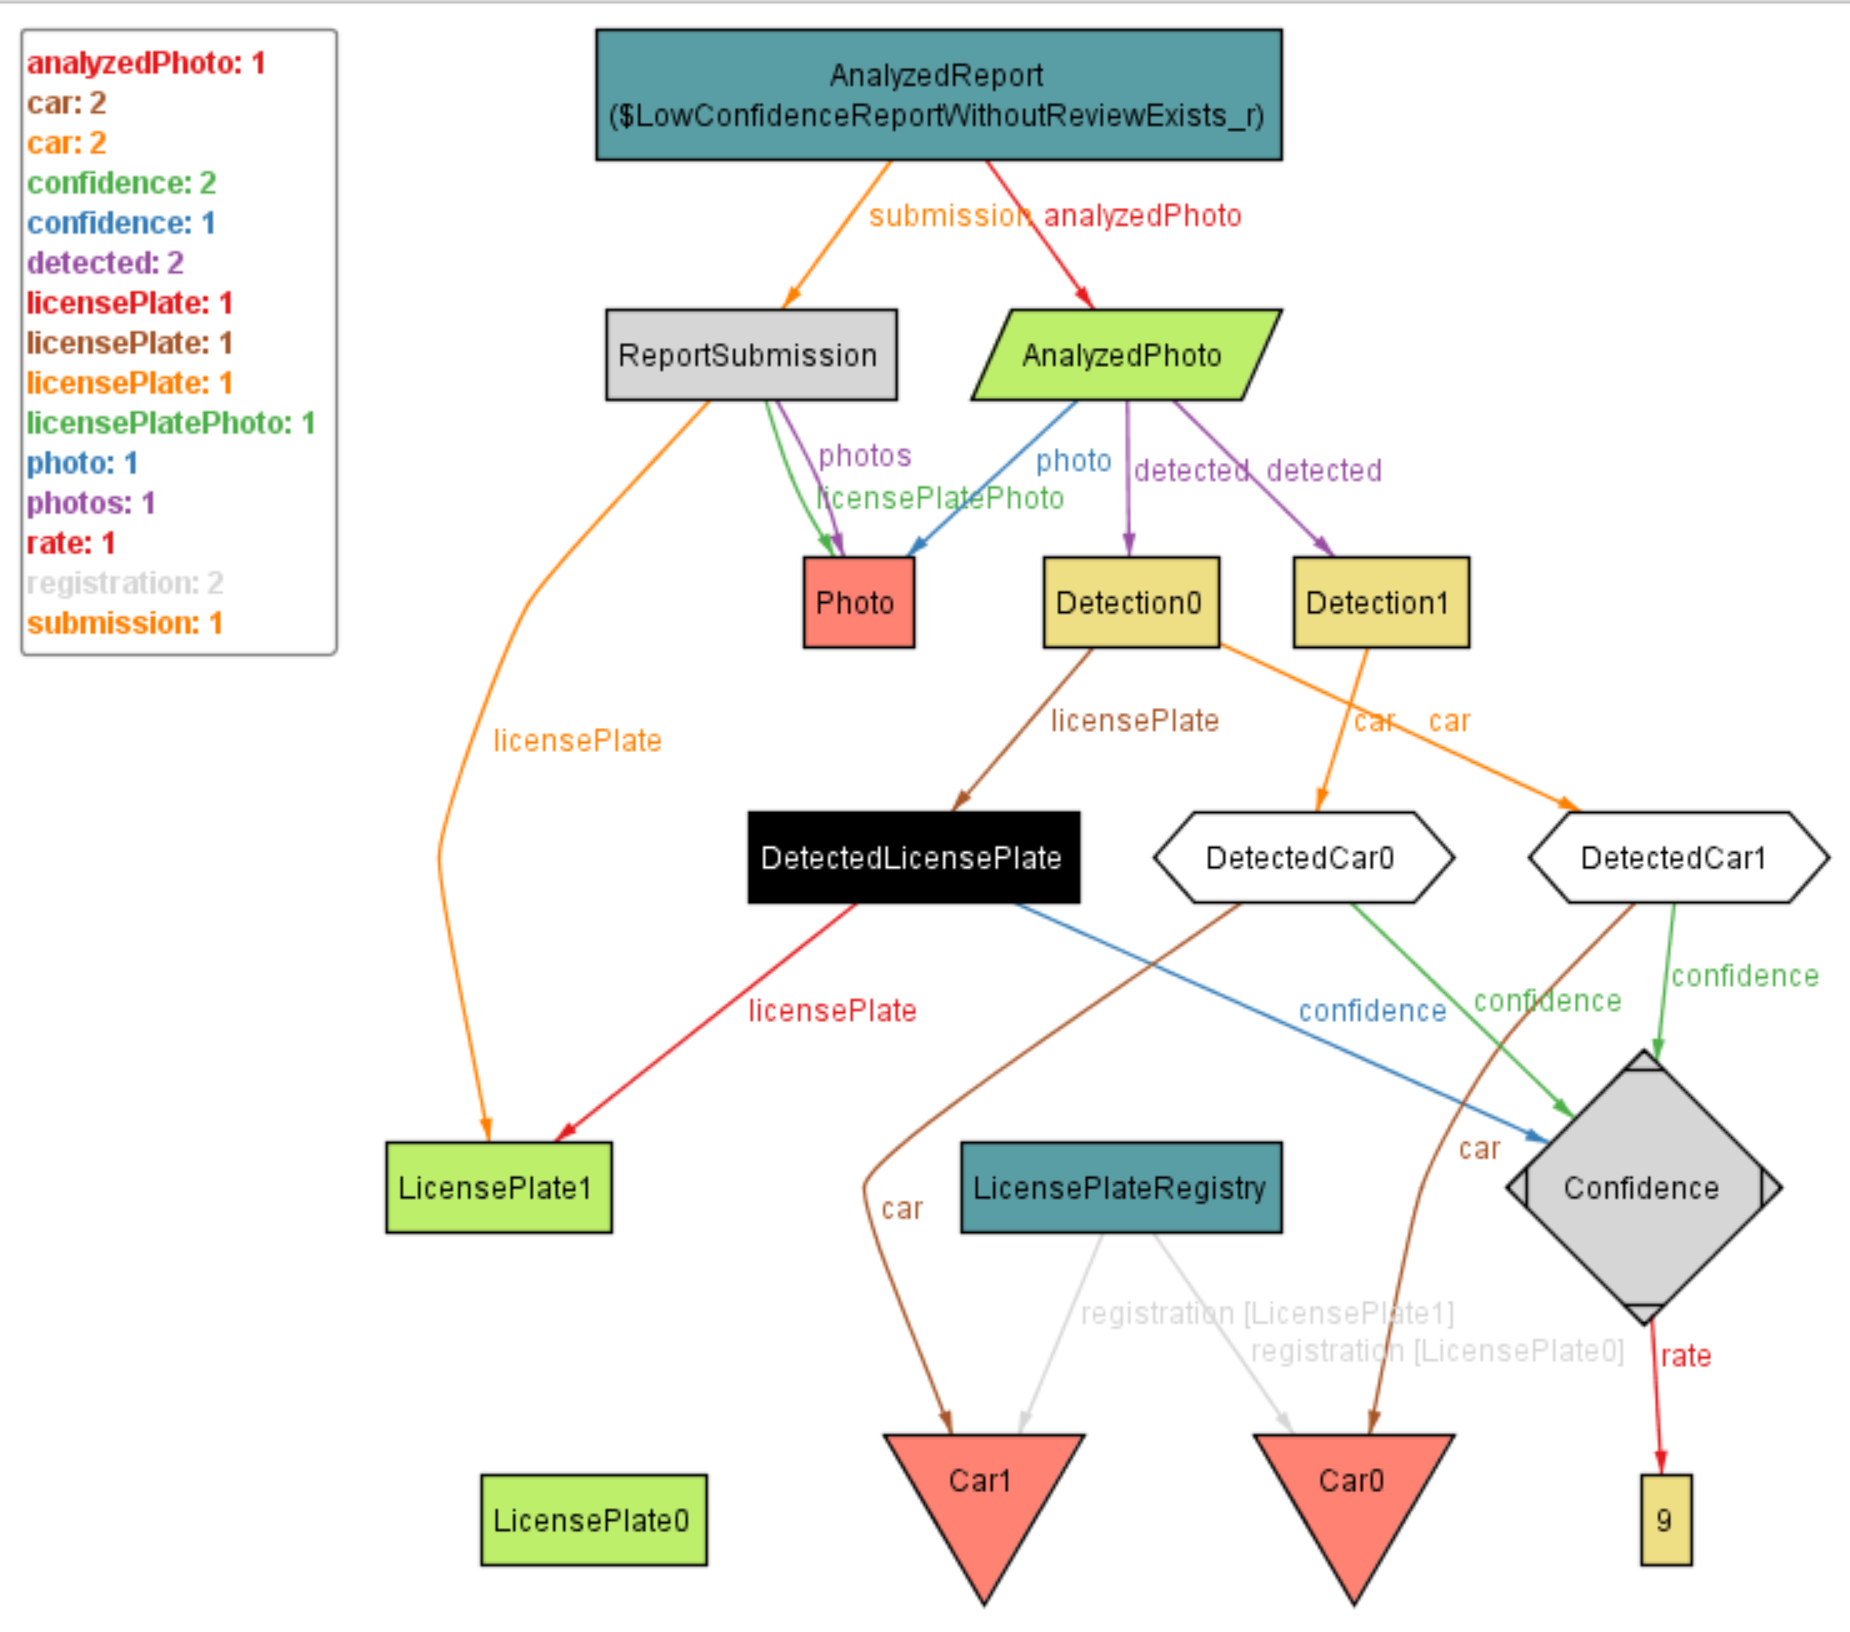
\includegraphics[width=\textwidth]{Images/alloy/8.png}
    \caption{\label{fig:alloy}Alloy - World: Low confidence report without a review.}
\end{figure}

\begin{figure}[H]
    \centering
    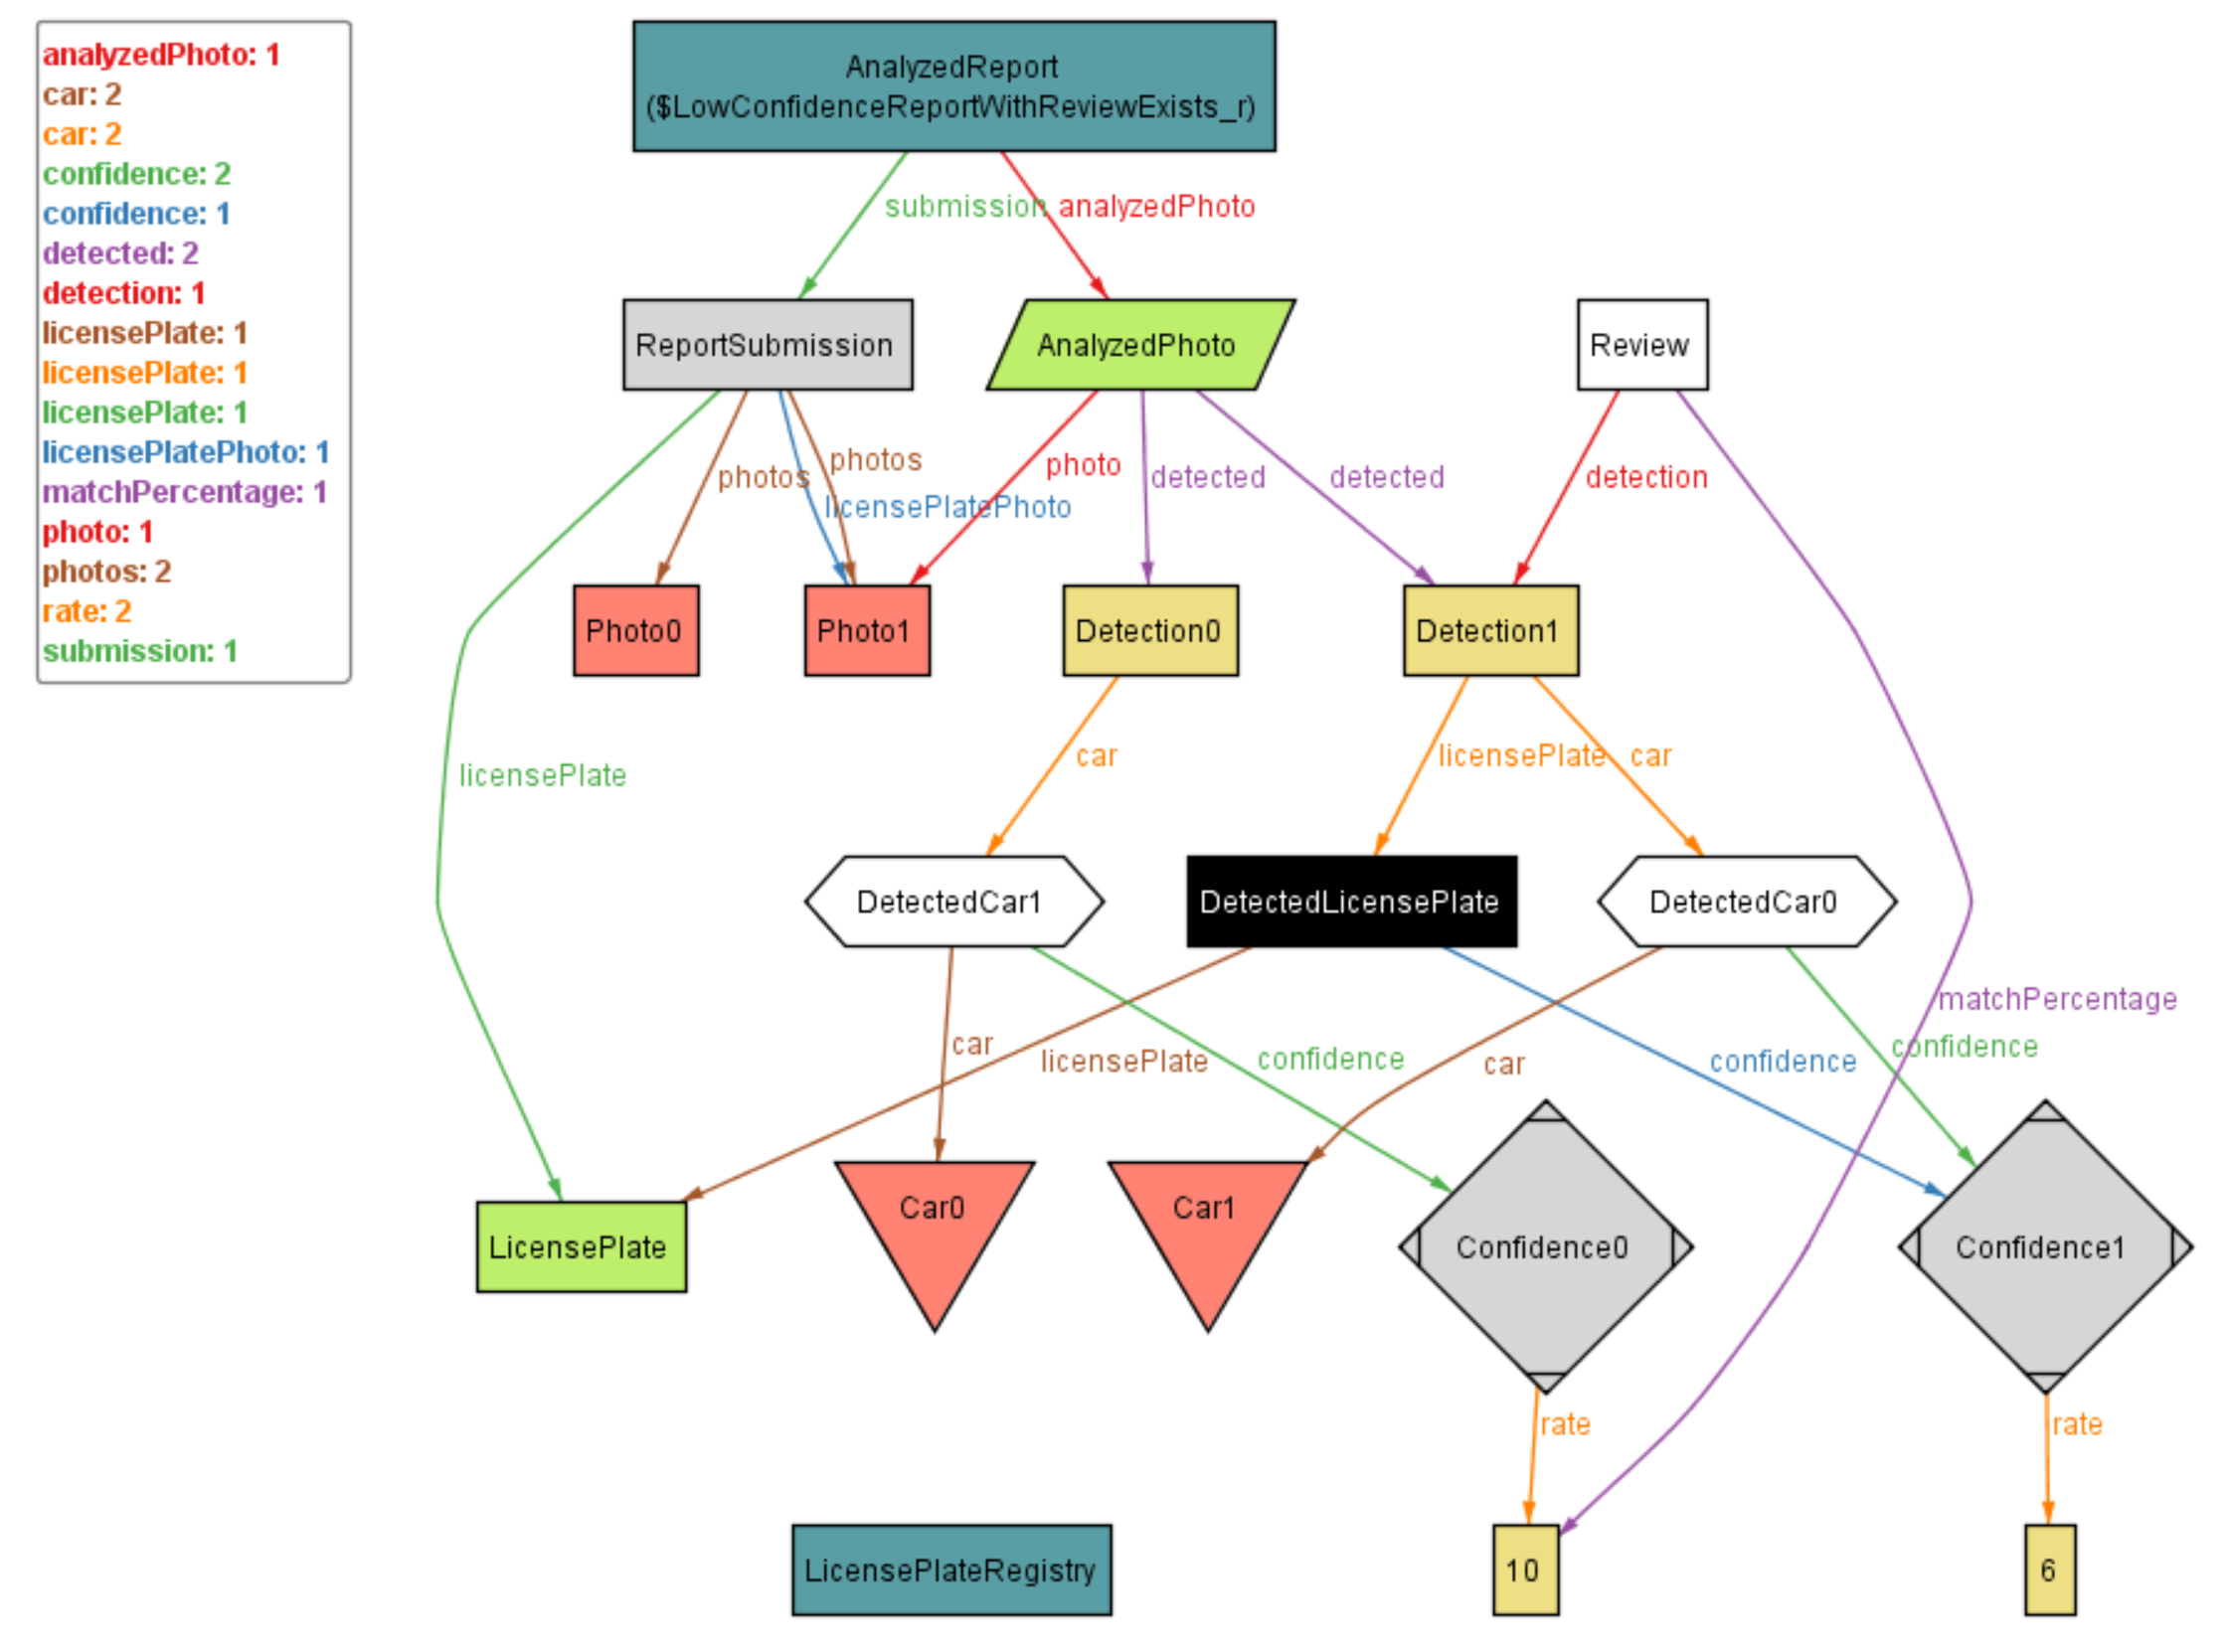
\includegraphics[width=\textwidth]{Images/alloy/9.png}
    \caption{\label{fig:alloy}Alloy - World: Low confidence report with a review.}
\end{figure}

\begin{figure}[H]
    \centering
    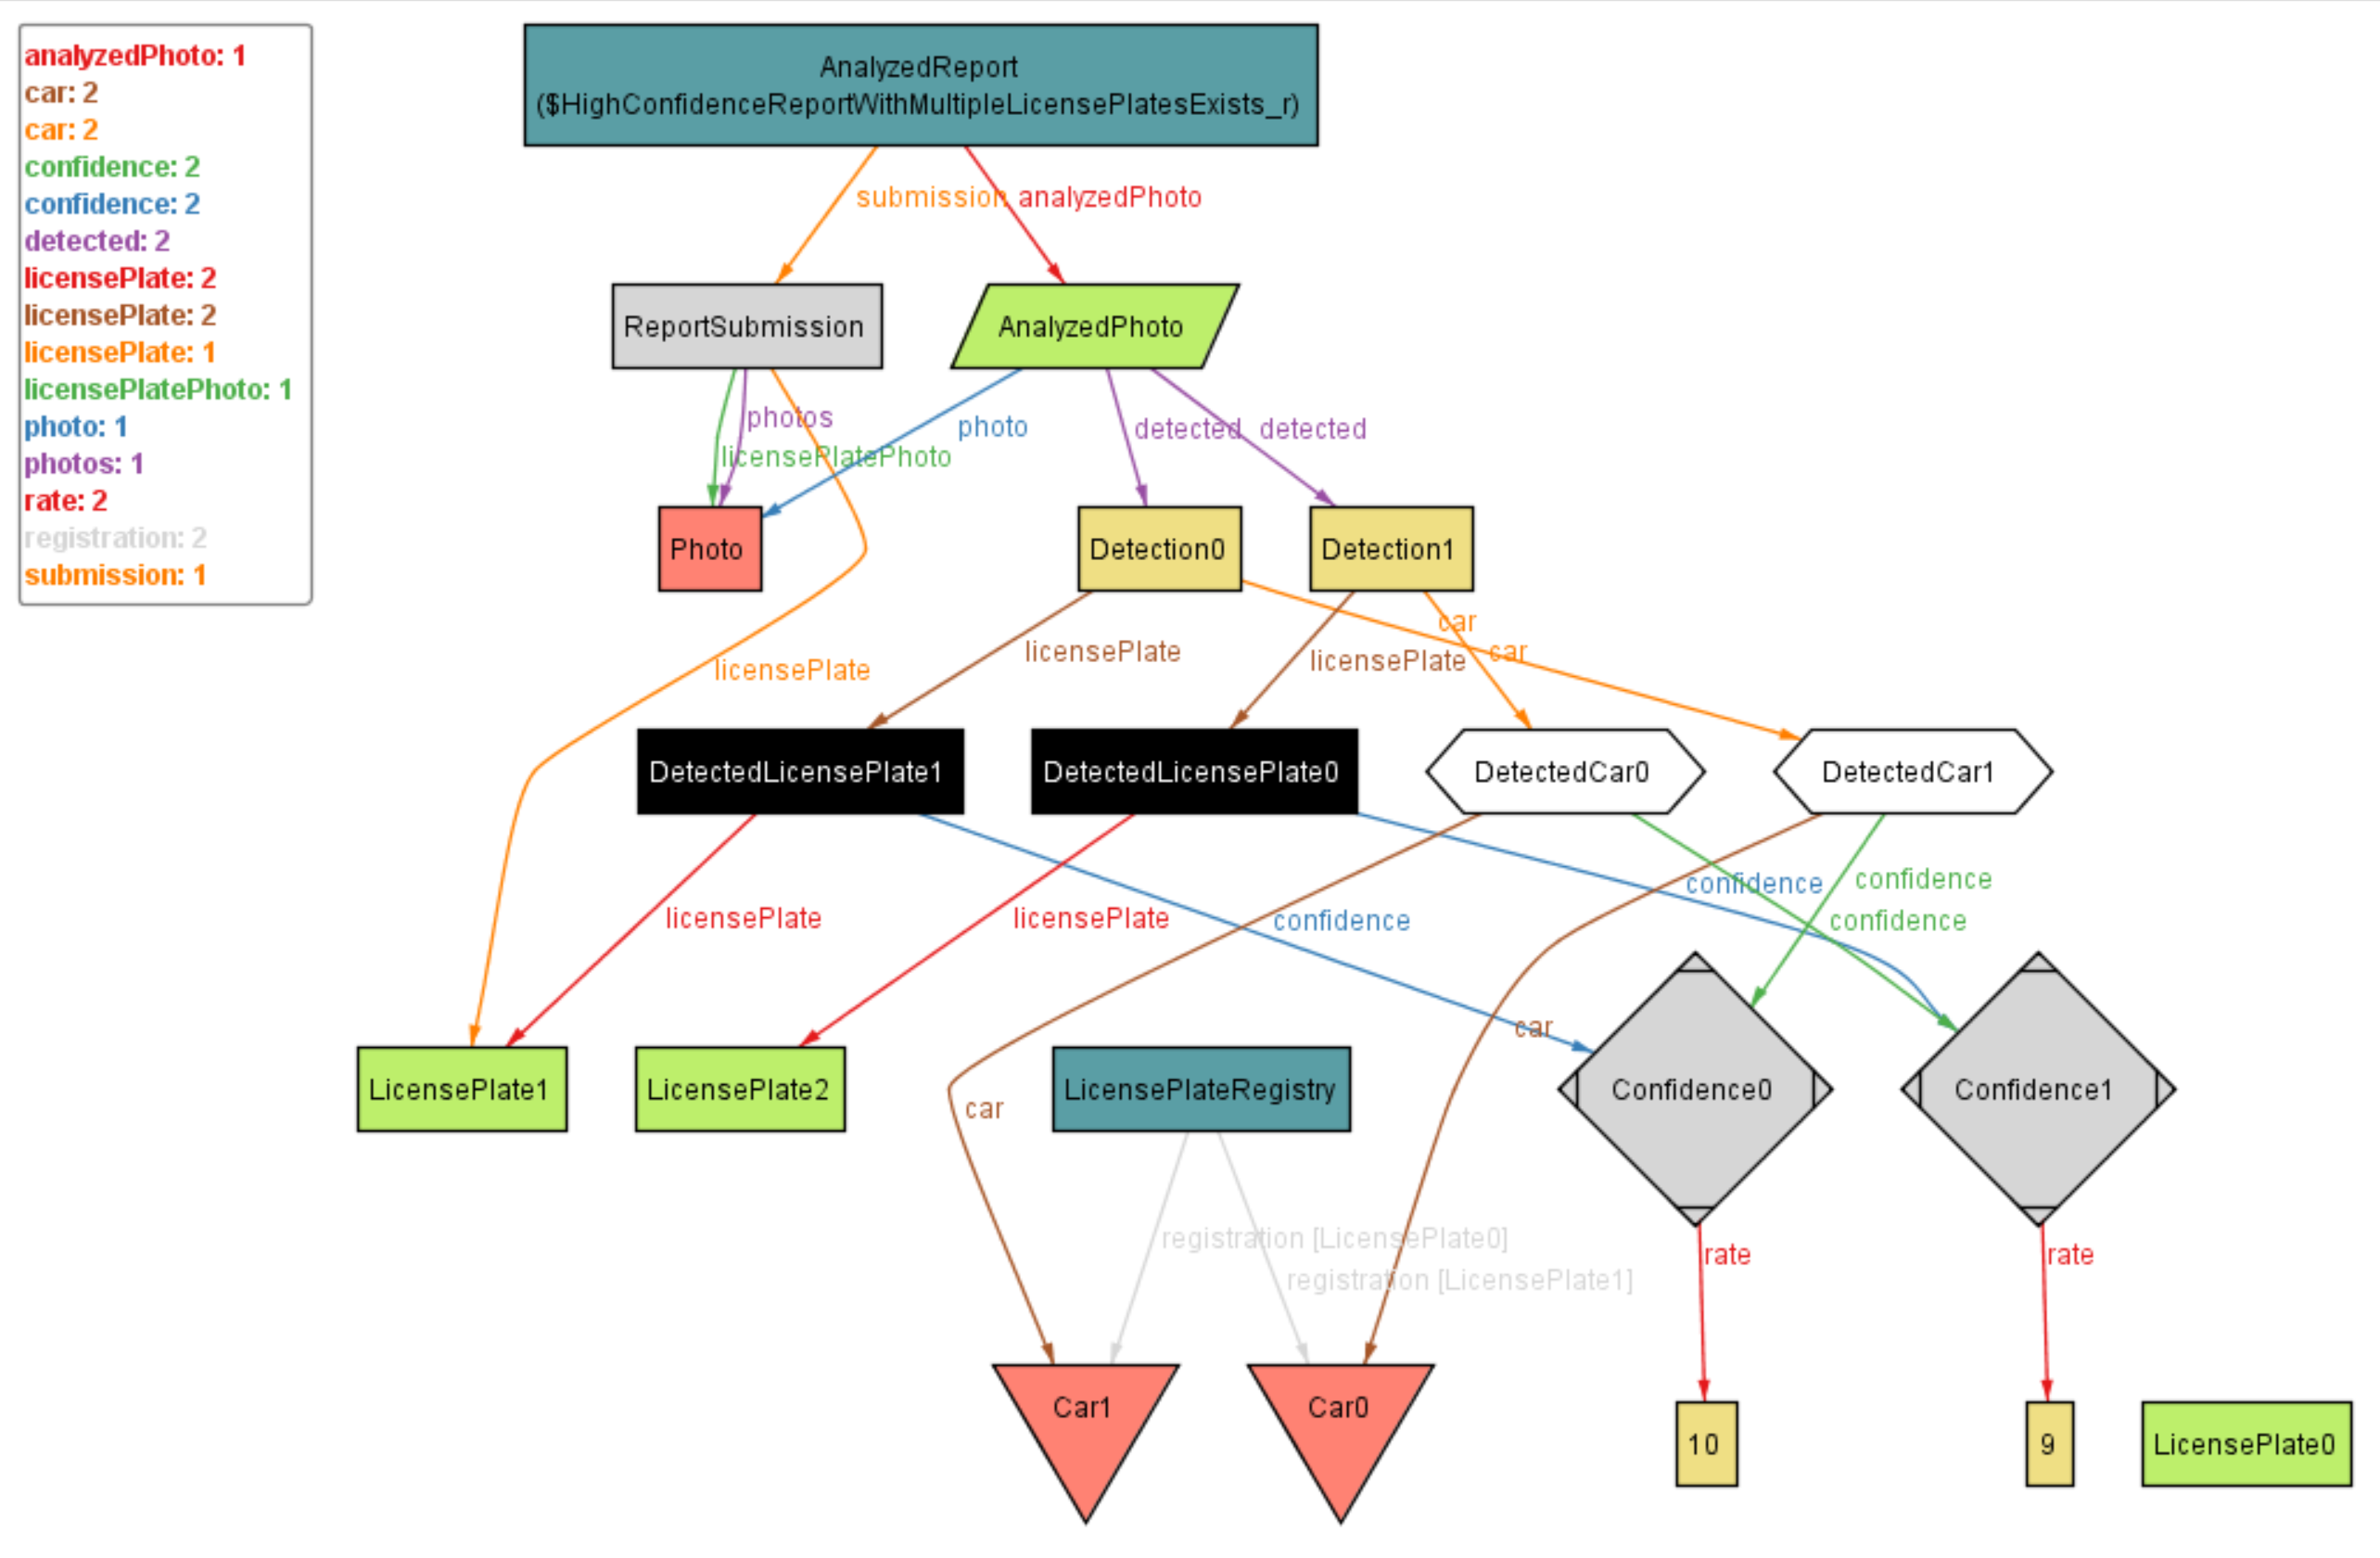
\includegraphics[width=\textwidth]{Images/alloy/10.png}
    \caption{\label{fig:alloy}Alloy - World: High confidence report with multiple license plates.}
\end{figure}

\begin{figure}[H]
    \centering
    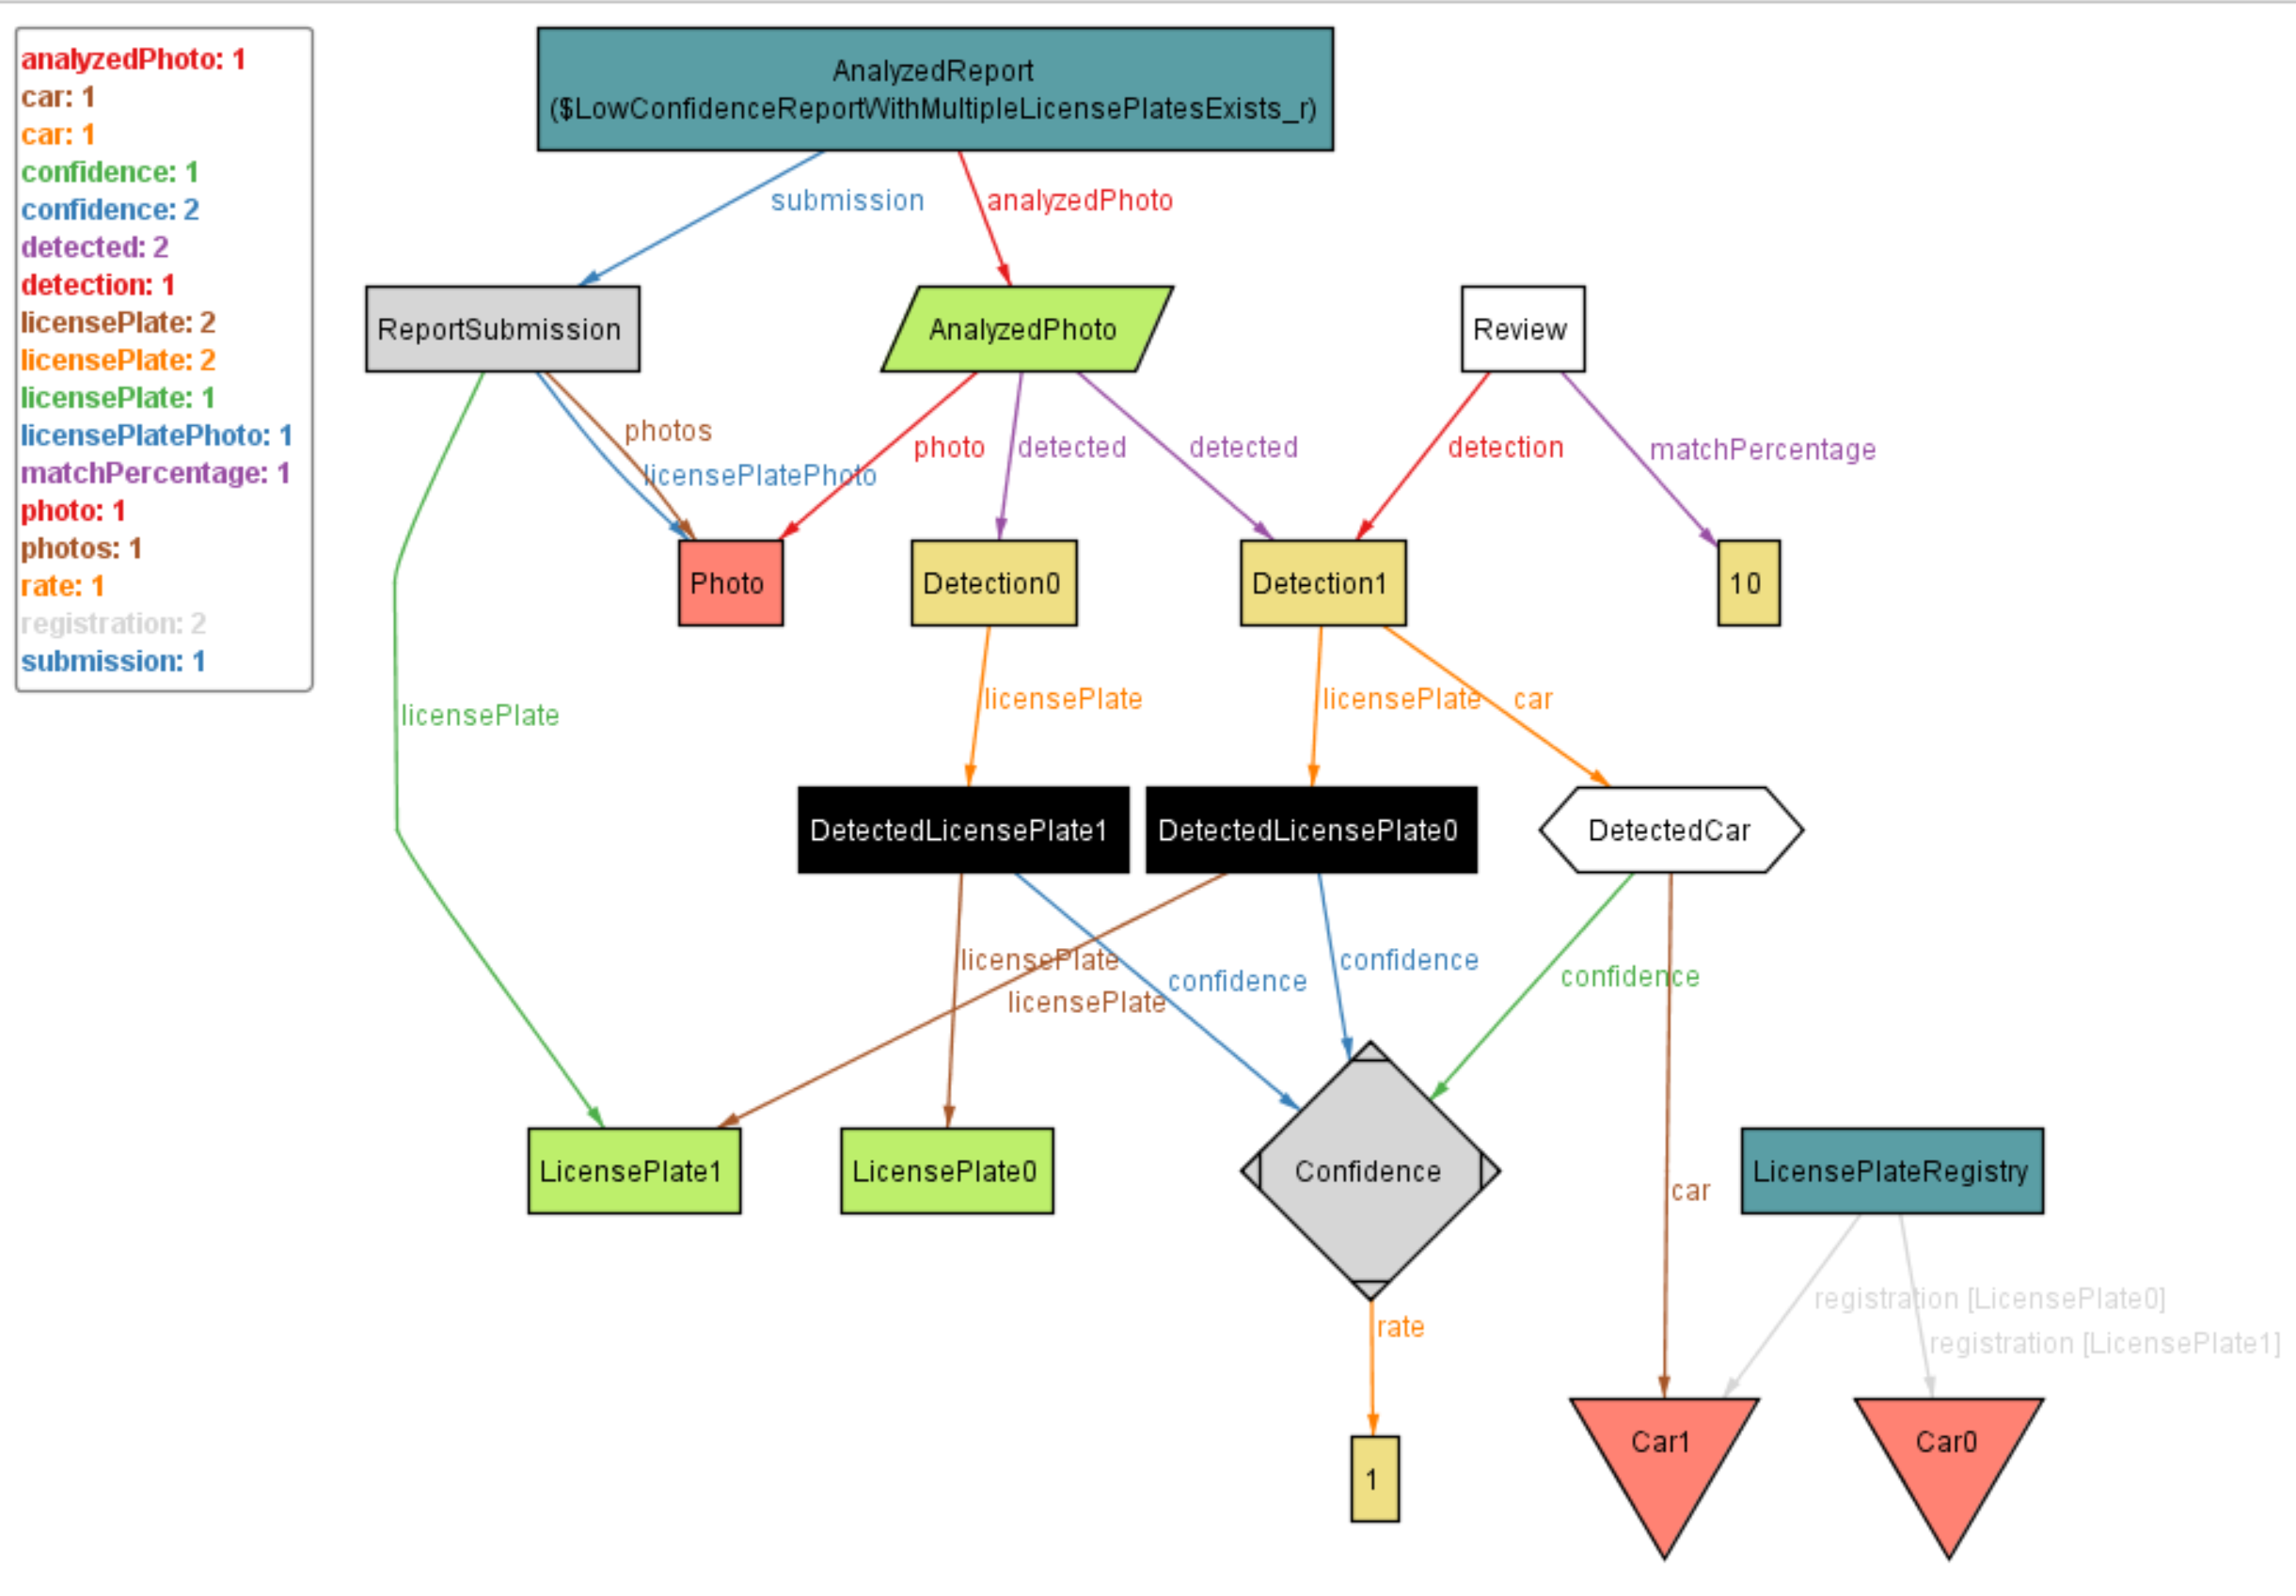
\includegraphics[width=\textwidth]{Images/alloy/11.png}
    \caption{\label{fig:alloy}Alloy - World: Low confidence report with multiple license plates.}
\end{figure}

\begin{figure}[H]
    \centering
    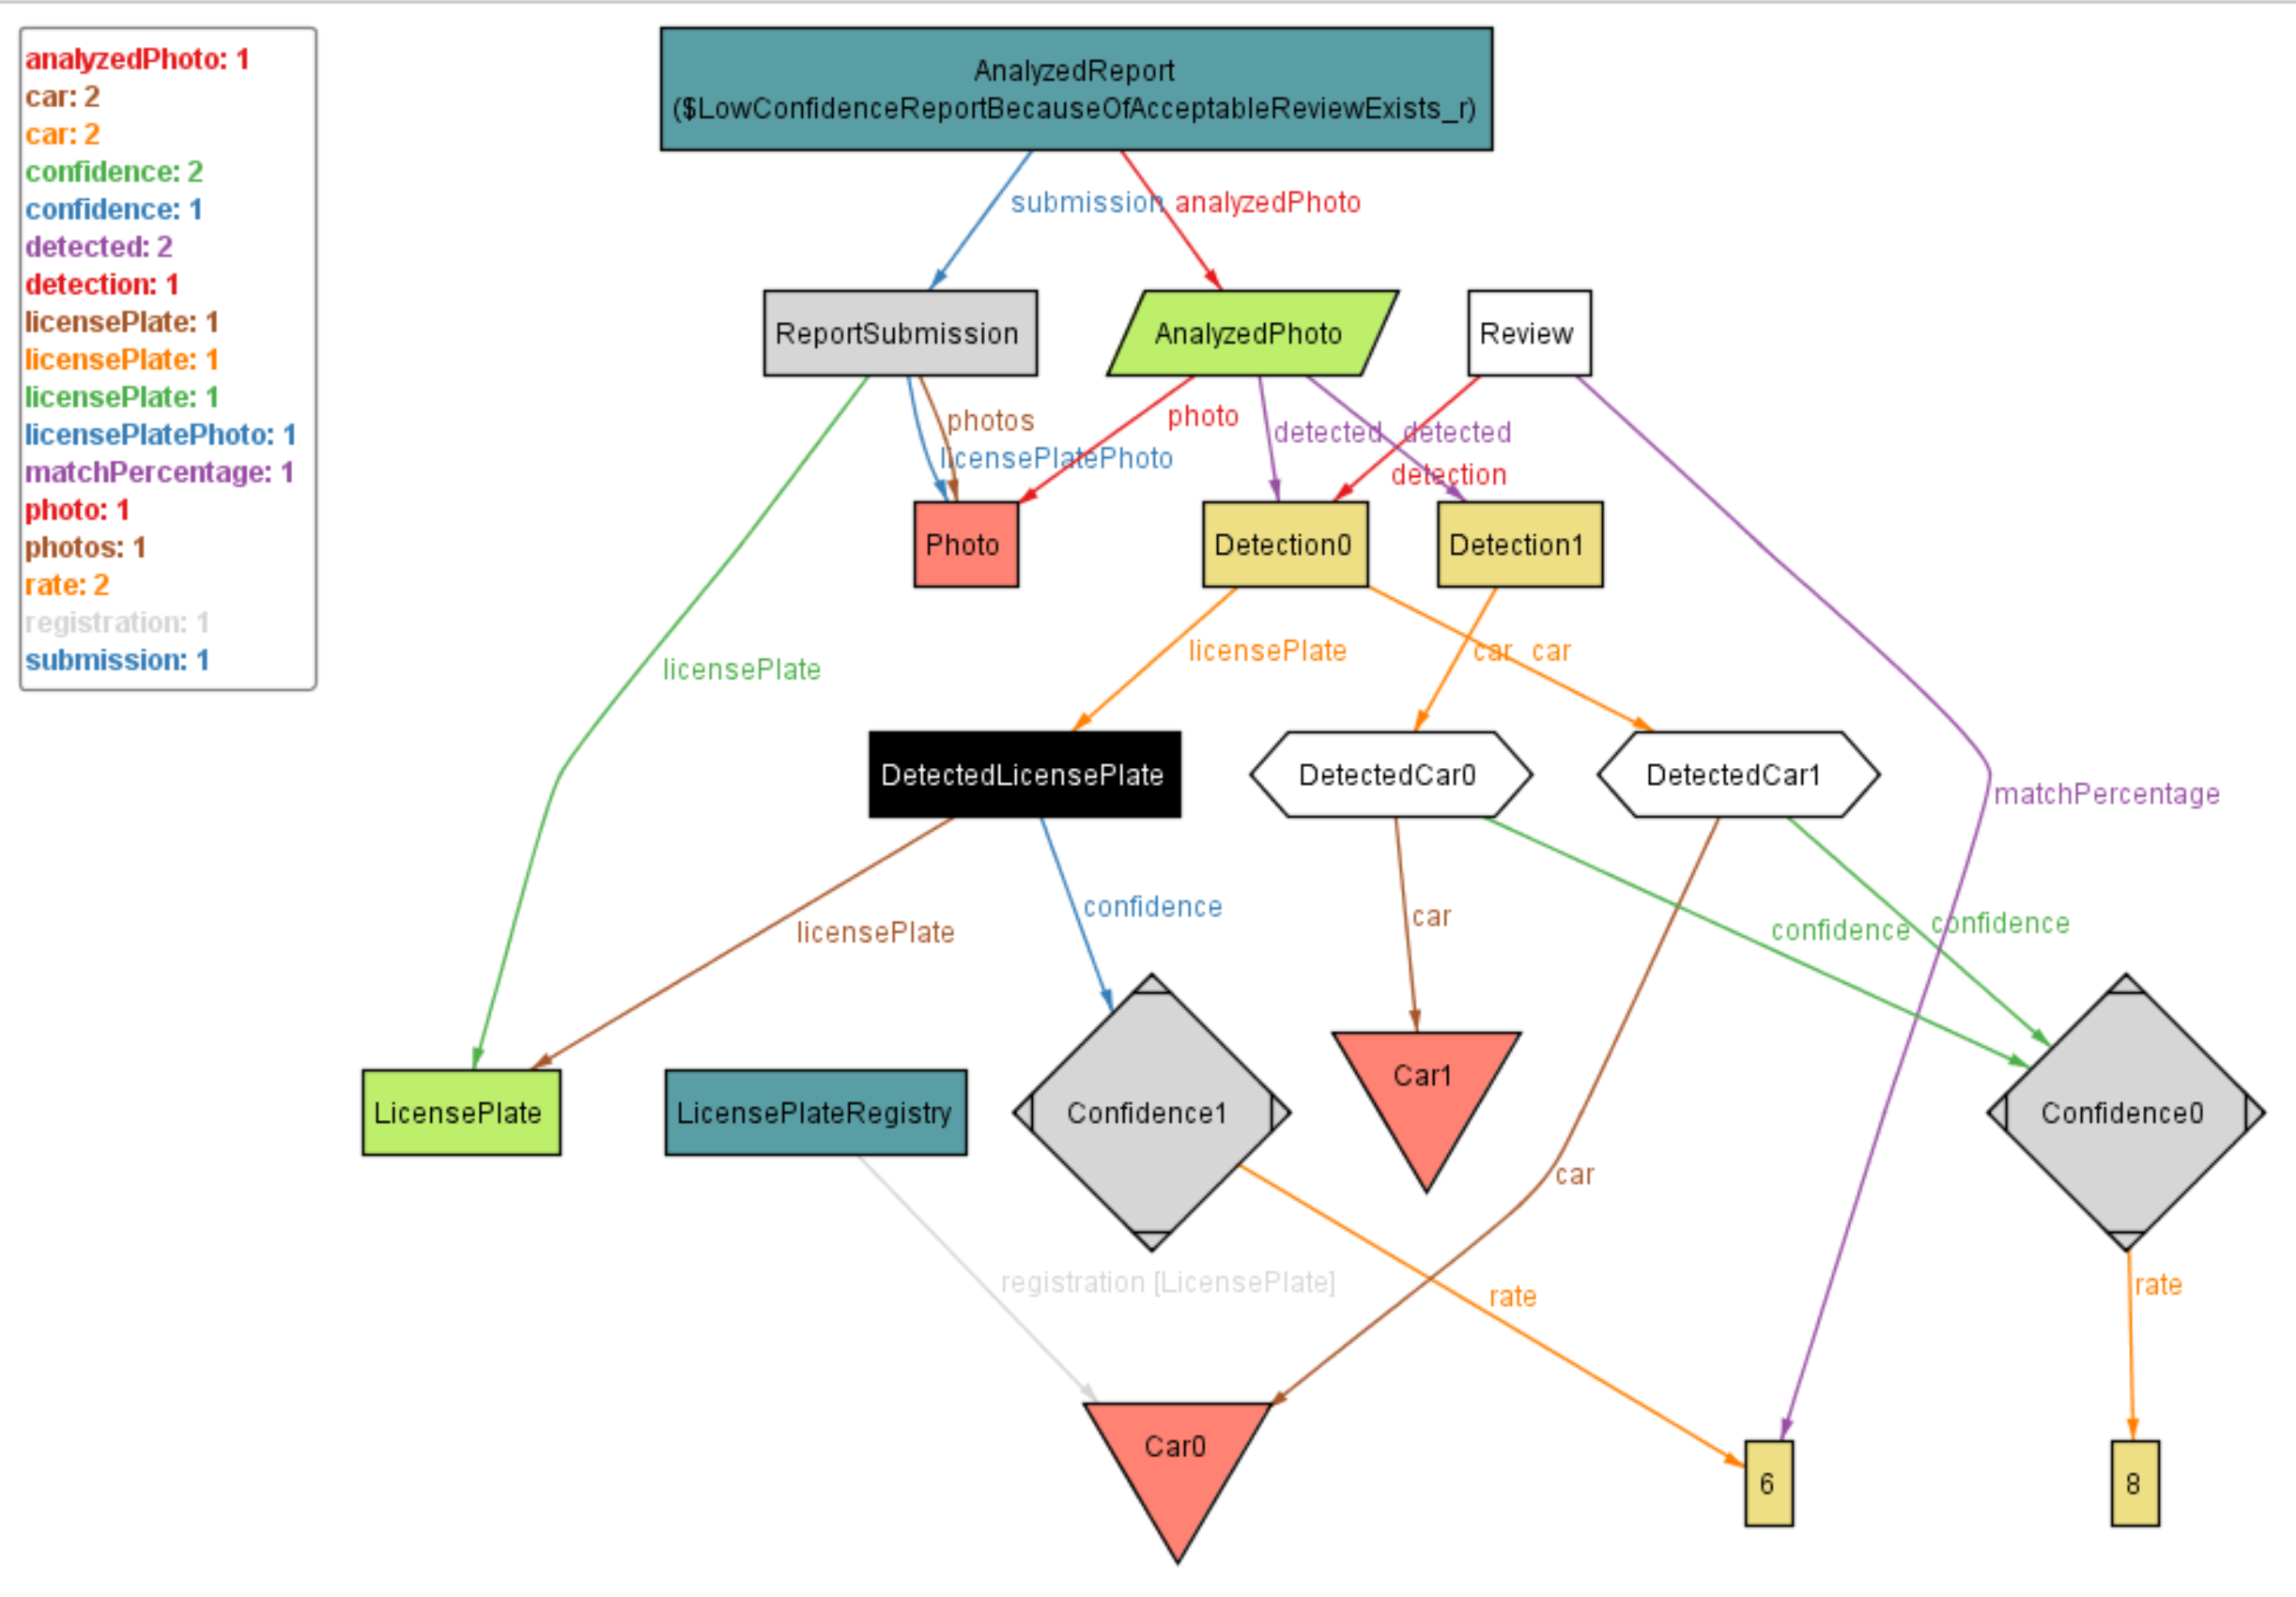
\includegraphics[width=\textwidth]{Images/alloy/12.png}
    \caption{\label{fig:alloy}Alloy - World: Low confidence report because of an "Acceptable" review.}
\end{figure}

\begin{figure}[H]
    \centering
    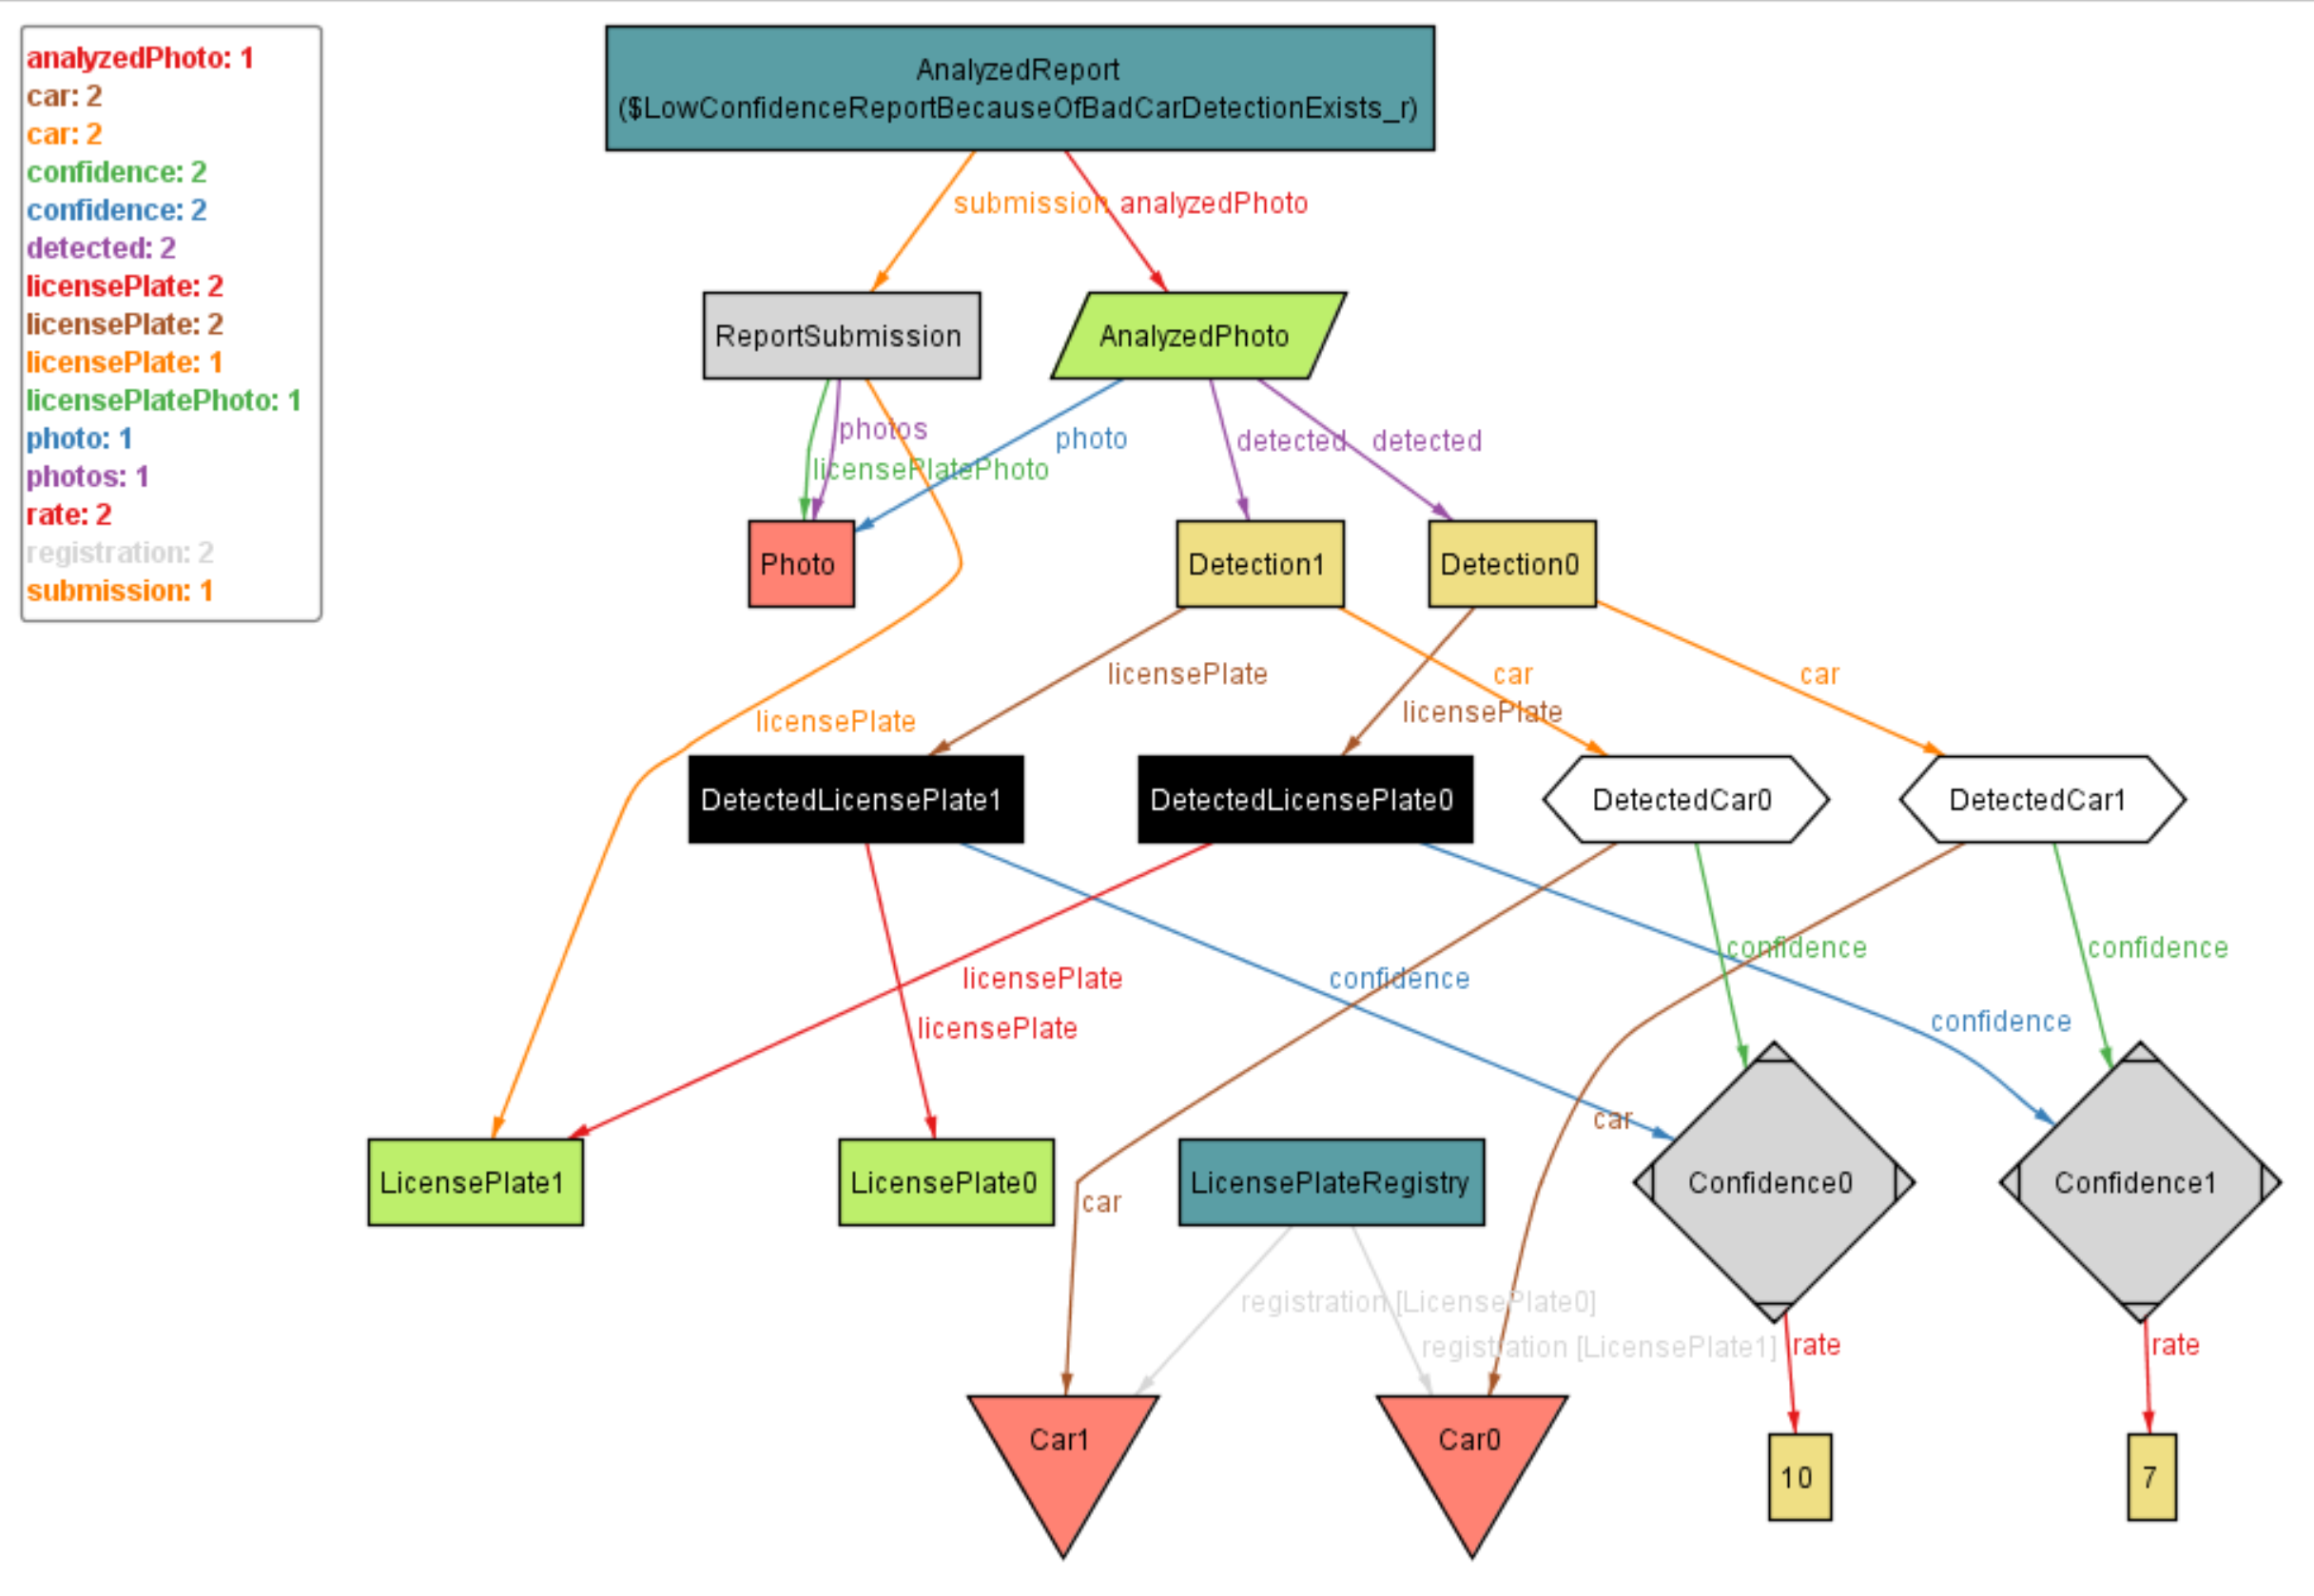
\includegraphics[width=\textwidth]{Images/alloy/13.png}
    \caption{\label{fig:alloy}Alloy - World: Low confidence report because of a bad car detection.}
\end{figure}

\begin{figure}[H]
    \centering
    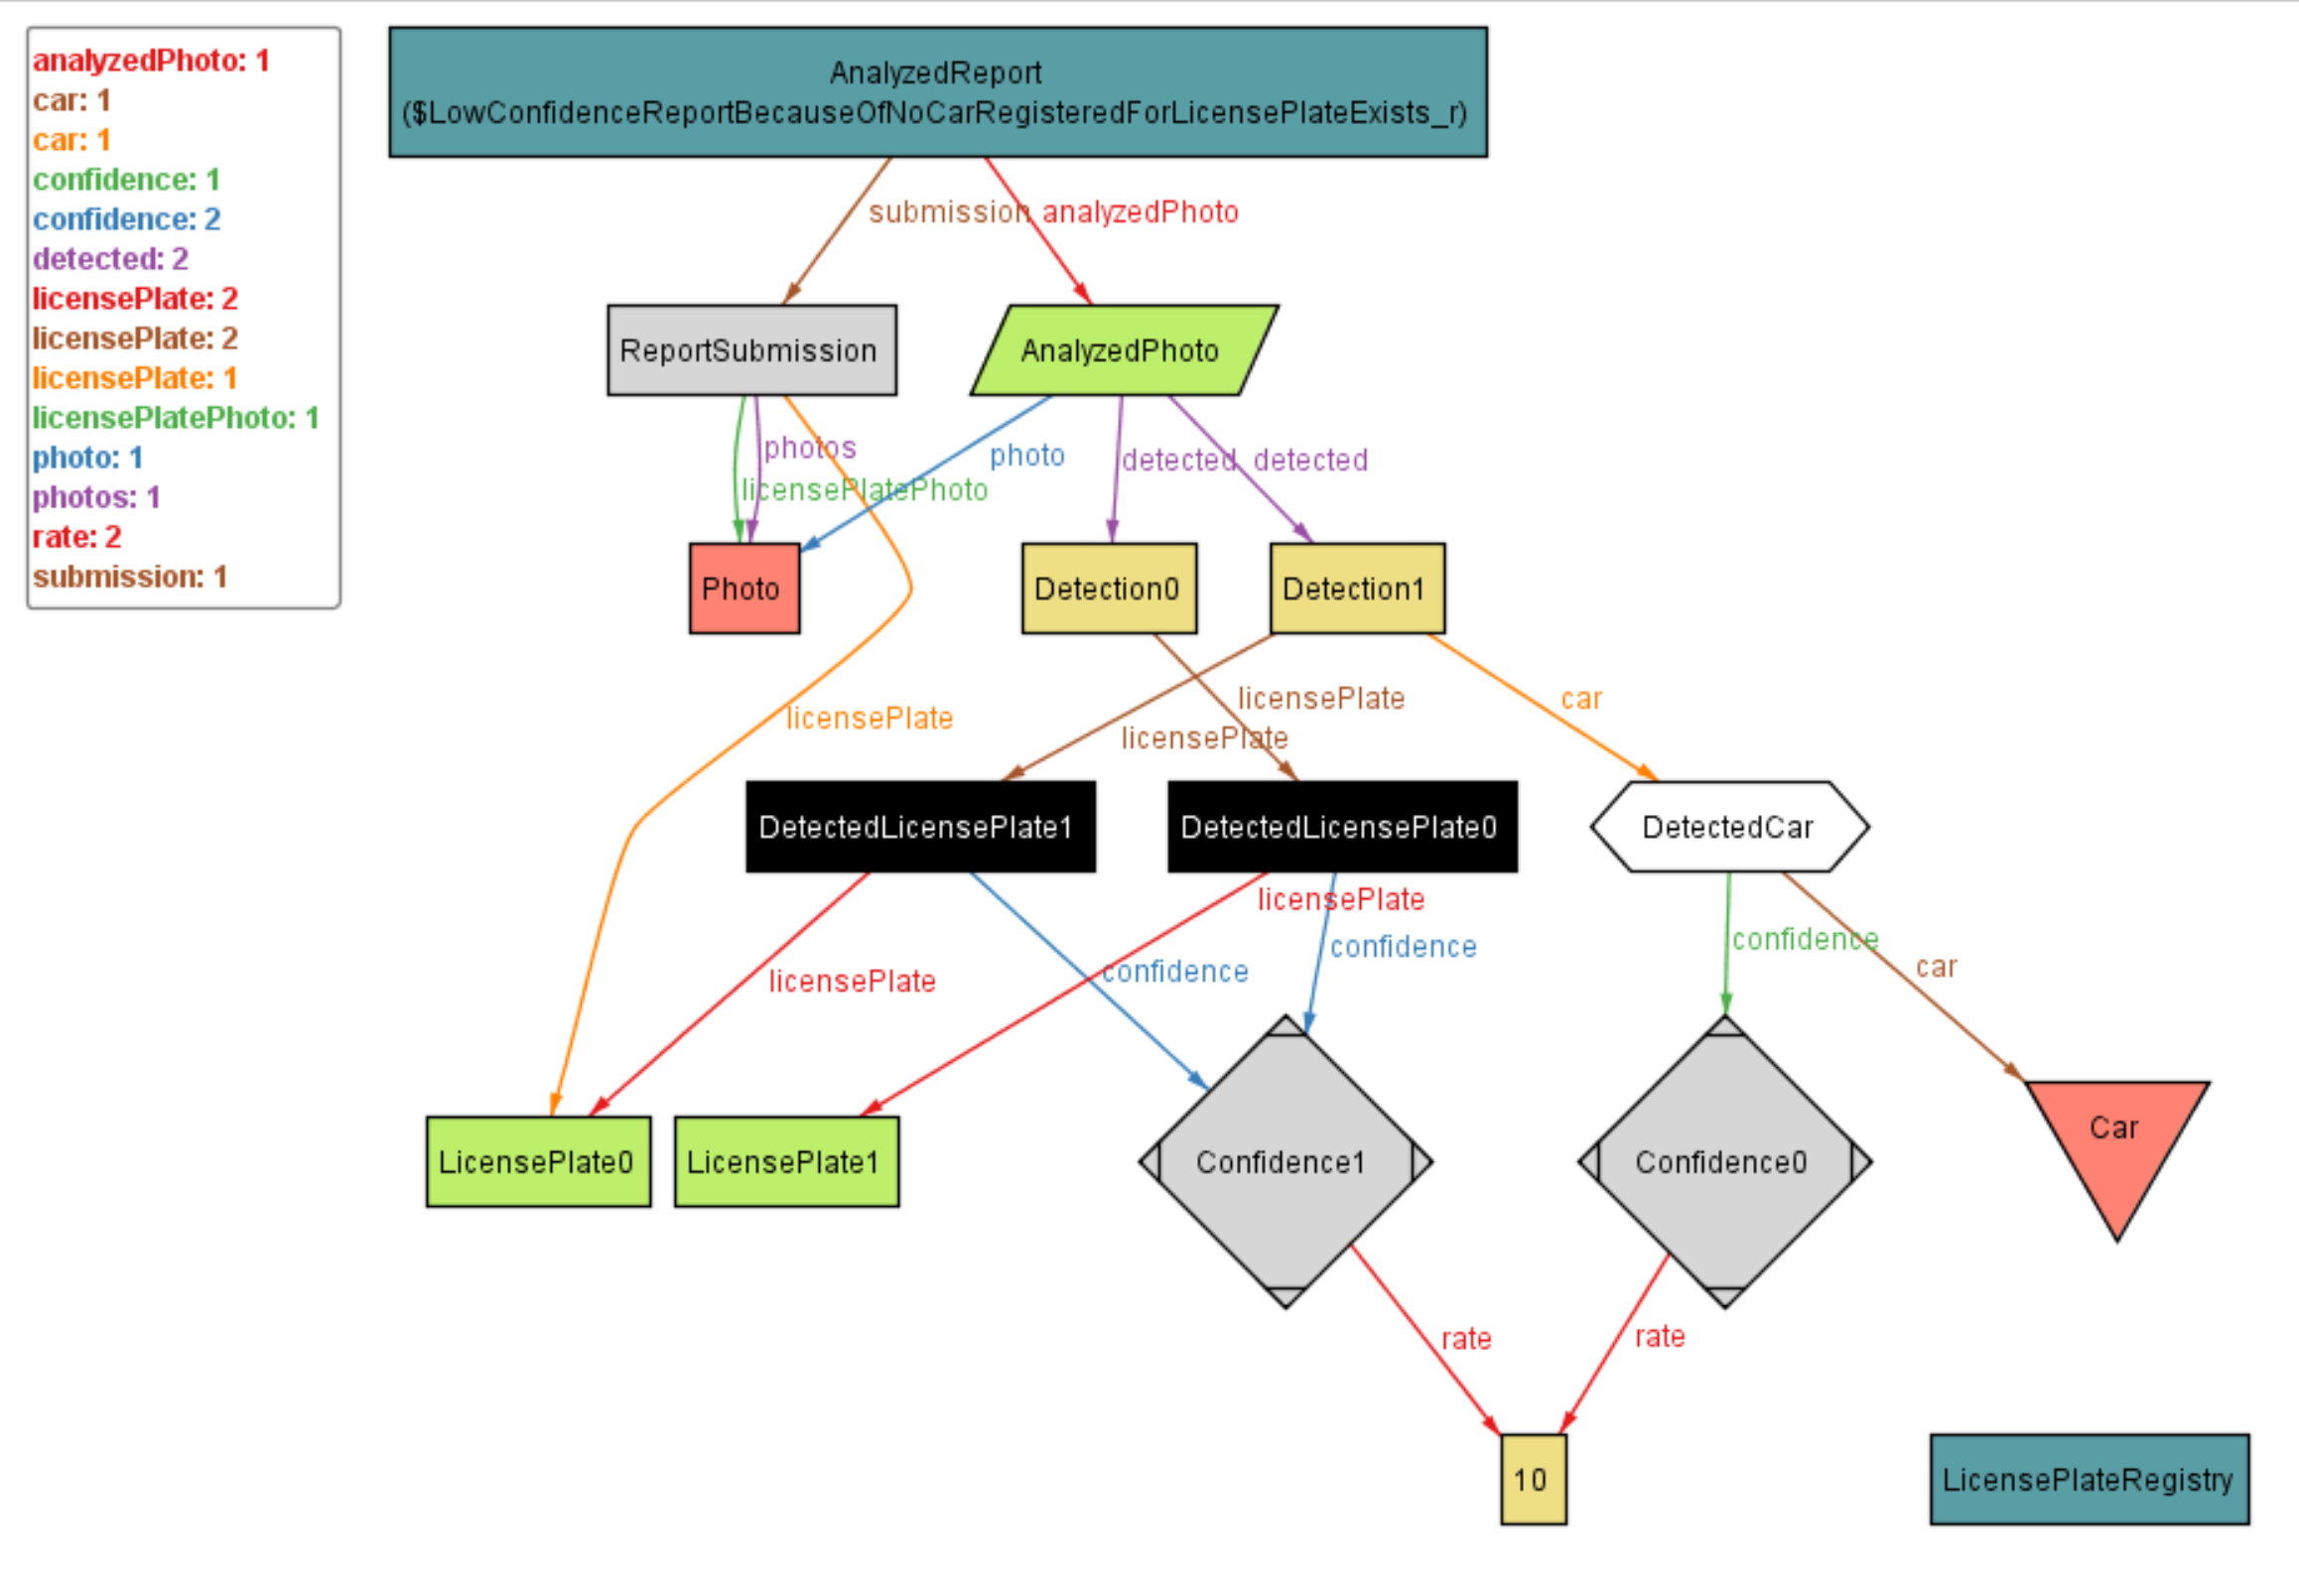
\includegraphics[width=\textwidth]{Images/alloy/14.png}
    \caption{\label{fig:alloy}Alloy - World: Low confidence report because there is no car registered under the detected license plate.}
\end{figure}

\begin{figure}[H]
    \centering
    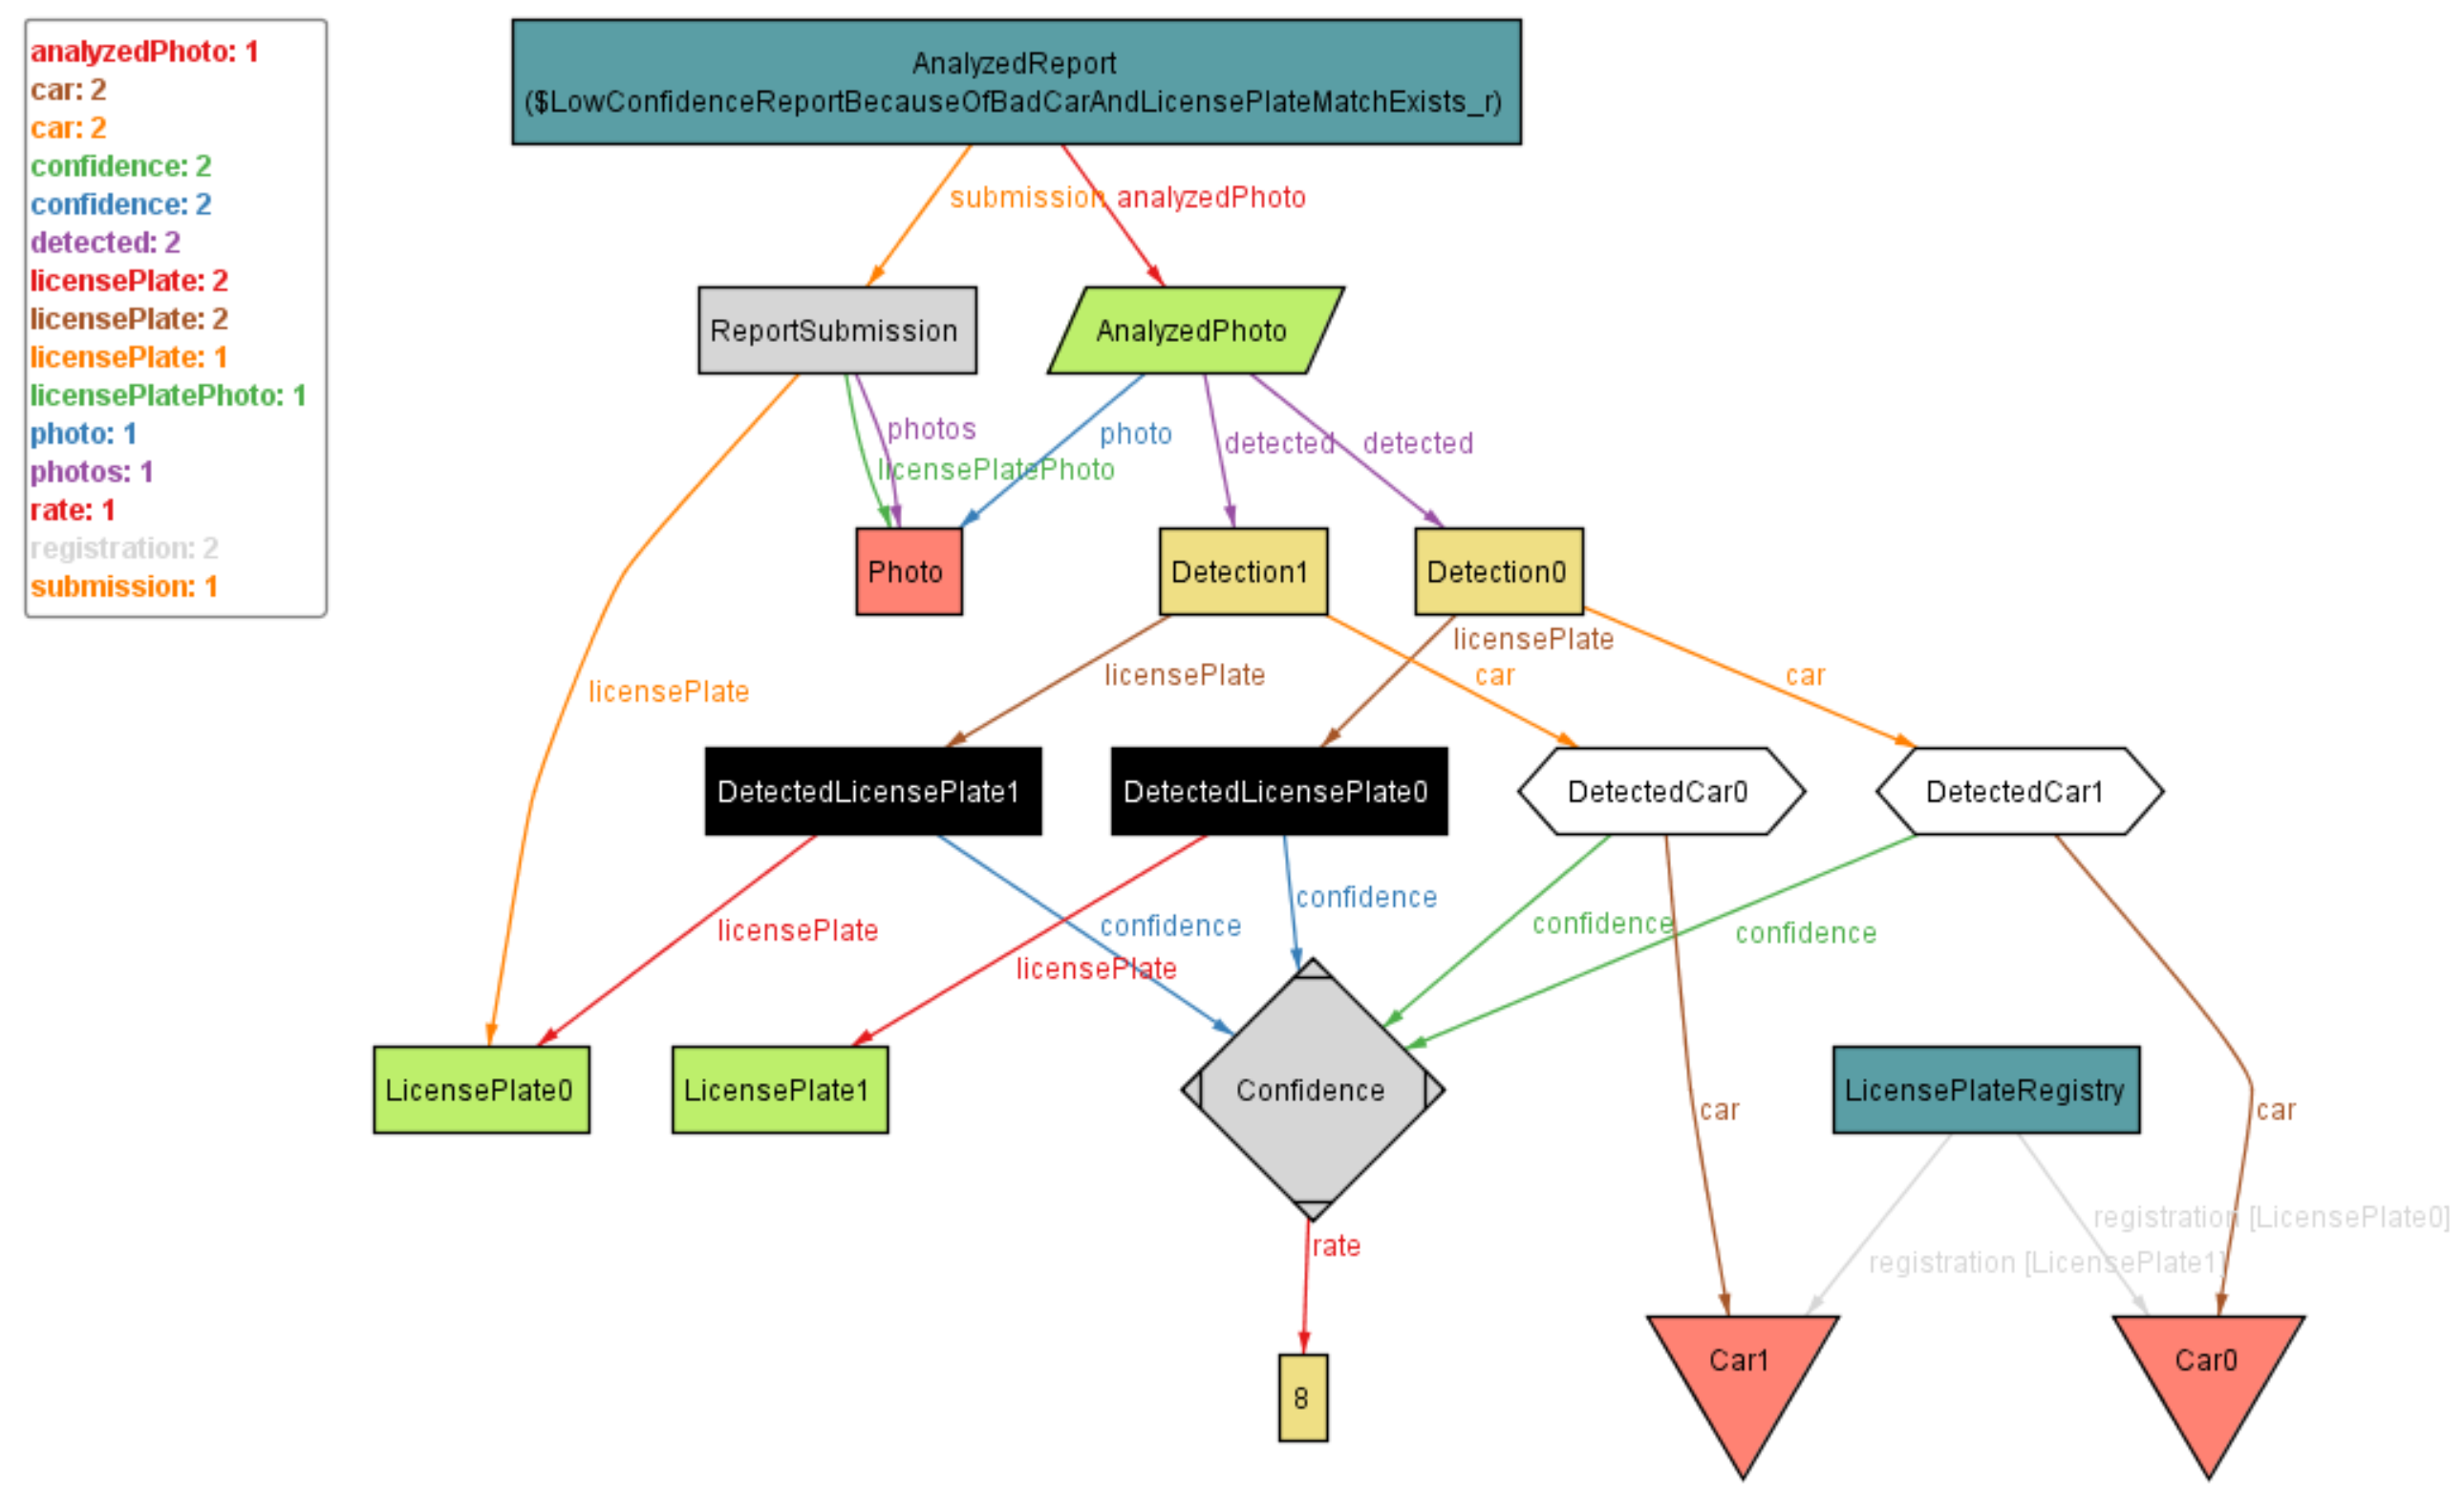
\includegraphics[width=\textwidth]{Images/alloy/15.png}
    \caption{\label{fig:alloy}Alloy - World: Low confidence report because the detected car does not match the car registered under the detected license plate.}
\end{figure}

